%!Tex Program = xelatex
\documentclass[a4paper,twoside,openright,notitlepage]{ctexbook}
%\documentclass[a4paper,fontset=none]{ctexbook}
%\ctexset{fontset=ubuntu} %设定CTeX宏包所采用的字体配置为ubuntu

\usepackage{xltxtra}
\usepackage{graphicx}
\usepackage{listings}
\usepackage{xcolor}
\usepackage{amssymb,amsfonts,amsmath,amsthm}
\usepackage[colorlinks,linkcolor=blue]{hyperref}
\usepackage{fancyhdr}
\usepackage{ulem}
\usepackage{array}
\usepackage{booktabs}
\usepackage{mathrsfs}
\usepackage{CJKfntef}

\lstdefinestyle{lfonts}{
basicstyle = \footnotesize\ttfamily,
stringstyle = \color{purple},
keywordstyle = \color{blue!60!black}\bfseries,
commentstyle = \color{olive}\scshape,
}
\lstdefinestyle{lnumbers}{
numbers = left,
numberstyle = \tiny,
numbersep = 1em,
firstnumber = 1,
stepnumber = 1,
}
\lstdefinestyle{llayout}{
breaklines = true,
tabsize = 2,
columns = flexible,
}
\lstdefinestyle{lgeometry}{
xleftmargin = 20pt,
xrightmargin = 0pt,
frame = tb,
framesep = \fboxsep,
framexleftmargin = 20pt,
}
\lstdefinestyle{lgeneral}{
style = lfonts,
style = lnumbers,
style = llayout,
style = lgeometry,
}
\lstdefinestyle{python}{
language = {Python},
style = lgeneral,
}


\newcounter{alg}[chapter]
\renewcommand{\thealg}{\arabic{chapter}.\arabic{alg}}

\newtheorem{definition}{定义}[chapter]

\newtheorem{theorem}{定理}[chapter]

\newtheorem{corollary}{推论}[chapter]

\newtheorem{example}{例}[chapter]

\renewcommand{\proofname}{\bf 证明}

%\setmainfont[Mapping=tex-text]{AR PL UMing CN:style=Light}
%\setmainfont[Mapping=tex-text]{AR PL UKai CN:style=Book}
%\setmainfont[Mapping=tex-text]{WenQuanYi Zen Hei:style=Regular}
%\setmainfont[Mapping=tex-text]{WenQuanYi Zen Hei Sharp:style=Regular}
%\setmainfont[Mapping=tex-text]{AR PL KaitiM GB:style=Regular} 
%\setmainfont[Mapping=tex-text]{AR PL SungtiL GB:style=Regular} 
%\newfontfamily\hei{WenQuanYi Micro Hei}
%\newfontfamily\whei{WenQuanYi Zen Hei}

\setCJKfamilyfont{kai}{KaiTi}
\newcommand{\kai}{\CJKfamily{kai}}
\setCJKfamilyfont{song}{SimSun}
\newcommand{\song}{\CJKfamily{song}}
\setCJKfamilyfont{fangsong}{FangSong}
\newcommand{\fs}{\CJKfamily{fangsong}}
\setCJKfamilyfont{hei}{SimHei}
\newcommand{\hei}{\CJKfamily{hei}}
\setCJKfamilyfont{lishu}{LiSu}
\newcommand{\lishu}{\CJKfamily{lishu}}

%\setmainfont[Mapping=tex-text]{Ubuntu}
%\setsansfont[Mapping=tex-text]{Ubuntu}
%\setmonofont[Mapping=tex-text]{Ubuntu}
%\setCJKmainfont[BoldFont = SimHei, ItalicFont = FangSong]{SimSun}

\renewcommand{\baselinestretch}{1.0}
\begin{document}
\pagestyle{empty}

\title{\hei 计算机模拟讲义}

\author{王何宇 \thanks{email:wangheyu@zju.edu.cn}\\
         数学科学学院\\
         浙江大学
       }
\maketitle
\thispagestyle{empty}

\pagestyle{headings}
\pagenumbering{Roman}

 
\tableofcontents

\chapter{概述}
\pagenumbering{arabic}

本课程主要讨论用如何计算机模拟随机事件,以及此为基础的优化算法、数值方
法和数学模型。随机,或者说不确定性,是我们所处世界的一个基本属性。而我
们人类,特别是受到过严格科学训练的人,其思维结构往往是偏向确定性的。这
就导致一部分人,甚至是受过高等数学教育的人,在对不确定性事物的直观理解
上,会有偏差。最常见的,比如赌徒心理:一个骰子如果已经连开十四次大,那
么它下一次开小的概率会不会上升?这个问题相对简单一点,我们来看一个更复
杂的游戏。

\section{例子:羊还是车 —— 对概率论结果的数值验证}
这个游戏最早来源于一个北美的电视节目,有点像综艺节目
\cite{Blues2016Edos}。最终环节主持人要来宾挑选礼物。礼物藏在三扇门后面,
两个门后面是一只山羊,而一扇门后面是一辆汽车。来宾知道礼物是什么,但不
清楚哪扇门后面是汽车。他只能随机打开一扇门,得到他的奖品。显然,汽车价
值要远高于山羊,所以来宾都更想得到汽车。主持人是知道哪扇门后是汽车的。
在来宾挑选了一扇门,尚未打开的时候,主持人会打开一扇藏了山羊的门(注意
  他总能做到这一点)。此时,来宾有一个选择,是坚持自己的门,还是换一扇?

\begin{figure}[!ht]
\centering
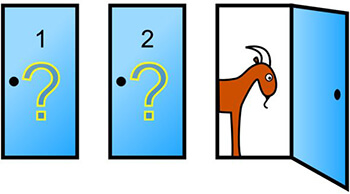
\includegraphics[width=0.7\textwidth]{images/game.jpg}
\caption{车还是羊?}
\label{fig::game}
\end{figure}

这个场景在电影《决胜21点》中也有出现。剧中男主角用概率论分析了这个问题:
``如果不换,那么选中车的概率就一直保持最初的$1/3$;而在主持人打开门以
后换一扇门,同时又能选中车的概率则是$2/3$。''我们知道好莱坞电影里的数学
理论大多数不那么严肃。那么这个主角也是在胡扯么?

选修了这门课的同学都不难自己用概率论验证,主角是正确的。但即便是一个严
格的概率论推导过程,真的就能真正说服我们么?是不是有一部分同学(甚至是
  大部分同学),始终觉得这就是在玩弄概率论。直觉上似乎始终有一个声音告
诉我们,一个确定的选择导致的已经发生的概率,不会因后续事件而改变。

对这件事情最好的回答,无过于我们真的去玩这个节目足够多的次数,比如
10000次,然后统计不同策略的得失。(注意是统计,这一点电影还是错了,它
  始终说是上面的分析是一个统计学过程,而事实上应该是概率论。真实的去数
  充分多的游戏中不同策略的结果,才是统计。统计就是数数字,而概率则是测
  度论。)于是我们首先需要10000辆车和20000只羊?如果谁愿意赞助我一定不
会反对。但更实际的,我们考虑一下能否在计算机中模拟这10000次游戏来达到
同样的统计结论。

为方便起见,在这门课中我选择Python 3.0来描述算法和实现程序。理由是这是
一门最接近自然语言和伪代码风格的语言。同时它又是大数据领域被广泛接受的
语言。我们不会专门讲述如何使用Python语言编程。而是在使用的过程中不断熟
悉这门语言。对于从未接触过Python的同学,我们会有一个简单的入门环节。可
能在上机课程或者以讲义的形式提供。

我们直接来读代码,Python的代码非常容易阅读。算法\ref{alg::game}给出了
用计算机模拟整个游戏的过程。并提供了simulation函数用于测试不同的策略,
并分别对两种策略进行了10000次模拟,统计了最终结果。一次典型的结果如下
(注意每次模拟的结果都会不同,如果是真随机的话):

\begin{lstlisting}
win rate of never exchange: 0.3357
win rate of exchange: 0.671
\end{lstlisting}

这个结果清晰的表明在``实际''游戏过程中,换与不换确实会有实质的不同。
概率论的结果并不是一个观点,而是客观事实。相反我们的直观并不一定总是正
确的。特别对于随机事件,我们要更加小心对待。最后让我们回到对概率论结果
的直观理解中。只要考虑一下,如果第一次选错的嘉宾,他在主持人开门之后换
一扇门一定可以得到车。而第一次选错的概率就是$2/3$。通过这个例子,我们
明白计算机模拟确实可以在我们发生怀疑的时候,帮助我们理解一个随机事件的
本质,即便已经有了概率估计,它也可以帮助我们建立正确的直观去理解概率结
果。

在这一过程中,真正起作用的是两件事情,第一是随机数的产生;第二是计
算机能够高效率地产生大量重复试验的结果,并可以对结果进行有效的统计。概
率论在这里确实是一个指导性思想。但我们的具体实现始终都是统计过程。这二
者能够达成一致的基本原理就是大数定律和中心极限定律。概率论是数学,它的
结论是客观事实。但如何理解是一个严重的问题。而统计实现过程也必须足够小
心。比如这个算法\ref{alg::game}大家觉得有没有严重的缺陷?使得它至多只
是一个模拟验证,而不能称为是一个数学结论。

问题就在于我们用计算机产生的``随机数''只能是伪随机数。它具备像一个真正
随机序列那样的分布特征,比如这里的随机数是均匀分布的,那么它在均匀性上
会表现的和真正的随机序列``几乎''一样。然而,它事实上是有规律的。这使得
我们一方面需要认真研究如何才能更高质量和高效率地产生伪随机数,另一方面
需要对这件事情有充分的认识,并在设计算法的时候小心谨慎。科研历史上确实
发生过由于伪随机序列的隐含规律导致模拟结果错误的事情。

\begin{minipage}[!ht]{0.8\textwidth}
\vspace{3ex}
\refstepcounter{alg}
\label{alg::game}
\begin{center}
 算法 \arabic{chapter}.\arabic{alg} 游戏:羊还是车
\end{center}
\small
\begin{tabular}{lll}
  \hei 输入&total&模拟的次数\\
  \hei 输出&&显示两种策略的胜率
\end{tabular}
\begin{lstlisting}[style = python, escapechar = \%]
def setup_game():
    # 三扇门初始化成都藏了羊。
    doors = [Prize.goat, Prize.goat, Prize.goat]
    # 先随机挑选一扇门,将羊换成车。
    car = np.random.randint(0, 3)
    doors[car] = Prize.car
    # 嘉宾挑选一扇门,然后主持人打开一扇藏有羊的门。
    guest = np.random.randint(0, 3)
    for host in range(0, 3):
        # 既不是藏有车的门,也不是嘉宾挑选的
        if host is not car and host is not guest:
            break
    return doors, guest, host

# 策略A, 打死也不换。这也是个函数,没毛病。
def strategyA():
    # do nothing.
    return

# 策略B, 换换更健康。
def strategyB(doors, guest, host):
    for new in range(0, 3):
        # 既不是之前挑选的门,也不是主持人打开的
        if new is not guest and new is not host:
            break
    return new

def simulation(total):
    # 嘉宾和主持人的选择,初始为-1。
    win = 0
    for i in range(total):
        doors, guest, host = setup_game()
        strategyA()
        if doors[guest] is Prize.car:
            win = win + 1
    print("win rate of never exchange:", win/total)
    win = 0
    for i in range(total):
        doors, guest,host = setup_game()
        guest = strategyB(doors, guest, host)
        if doors[guest] is Prize.car:
            win = win + 1
    print("win rate of exchange:", win/total)
    return
\end{lstlisting}
\end{minipage}

\section{随机优化算法简介}
除了对一个随机事件进行直接模拟。随机算法还可以用在优化求解上。这一类算
法经常被归入Monte Carlo方法,也有人将其进一步分化成Monte Carlo方法和
Las Vegas方法。它们分别代表了两种侧重略有区别的策略。不太严格地说,对
一个优化问题
\begin{equation}
\min f(x), x \in \mathcal{D}. 
\label{eq::min}
\end{equation}
这里$\mathcal{D} \in \mathbb{R}^m$是问题的定义域, $m$是维数. Monte
Carlo法的思路是在$\mathcal{D}$中以某种分布进行随机采样$\xi \in
\mathcal{D}$, 并根据$f(\xi)$的结果不断调整分布. 然后随着采样次数$n$
的增多,有
$$
\lim_{n \to \infty}E(\xi) \stackrel{1}{\hookrightarrow} x^*.
$$其中$x^*$是问题(\ref{eq::min})的真解。而Las Vegas方法则不停地随机投
点并根据反馈调整分布,直到在某一次测试中,发现$\xi$严格地等于$x^*$才能
结束。显然,Las Vegas方法可以看作是Monte Carlo方法的一个特例。而且它更
加适用于离散优化。我们在之后的讨论中不再区分二者。

Monte Carlo法的实际应用也远比优化要宽广。理论上它几乎可以解决任何问题
(在不计效率的前提下)。下面给一个几乎所有Monte Carlo讲义都会提到的例
子,计算圆面积.

\begin{figure}[!ht]
\centering
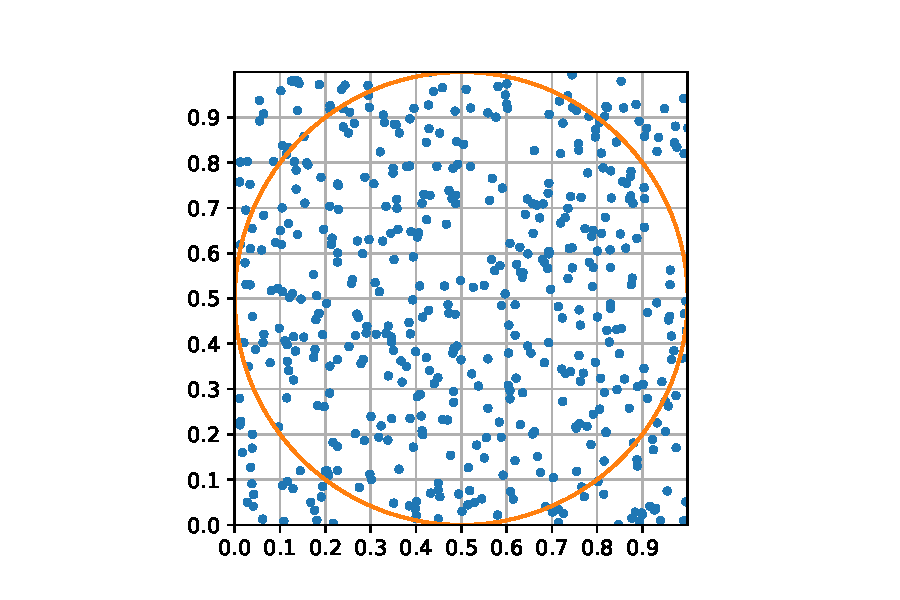
\includegraphics[width=0.7\textwidth]{images/circle.pdf}
\caption{求圆面积}
\label{fig::circle}
\end{figure}

如图\ref{fig::circle},我们通过随机投点来估计这个内接在单位正方形内部
的单位圆的面积。我们要确保每一次投点都是满足在单位正方形内均匀分布的,
这样点落在圆内的概率$p$就是圆面积和正方形面积之比。因此我们只要统计落
在圆内和落在圆外的点的数目,那么它们二者之比就会在大数定律的控制下依概
率收敛到$p$。这样就可以计算出圆面积。我们在今后的学习中会用严格的概率
理论重建这个过程,而现在先用朴素的语言描述以便于直观理解,好在具体的算
法和程序过程仍然是严格的。

\begin{minipage}[!ht]{0.8\textwidth}
\vspace{3ex}
\refstepcounter{alg}
\label{alg::circle}
\begin{center}
 算法 \arabic{chapter}.\arabic{alg} Monte Carlo法求圆面积
\end{center}
\small
\begin{tabular}{lll}
  \hei 输入&times&抽样次数\\
  \hei 输出&&圆面积的计算值
\end{tabular}
\begin{lstlisting}[style = python, escapechar = \%]
def area_circle(times):
    inside = 0
    dots = np.random.rand(2, times)
    for i in range(times):
        x = dots[0, i] - 0.5
        y = dots[1, i] - 0.5
        if x * x + y * y < 0.25:
            inside += 1
    return inside / times
\end{lstlisting}
\end{minipage}

%% 积分的例子,即求
%% \begin{equation}
%%   I = \int_\mathcal{D}f(x) dx, \mathcal{D} \in \mathbb{R}^m.
%% \label{eq::int}
%% \end{equation}
%% 这里如果$f(x) = 1$, 则问题就是求$m$区域$\mathcal{D}$的测度。比如$m =
%% 2$就是求$\mathcal{D}$的面积。我们来看一个特例:
%% \begin{equation}
%%   I = \int_0^1f(x) dx, \mathcal{D} \in \mathbb{R}^m.
%% \end{equation}

由于我们在计算圆面积的时候没有使用圆面积公式。因此实际上我们可以通过这
个程序来估计$\pi$值。这个其实不是我们接触到的第一个求圆周率的随机算法。
大家还记得上概率论时介绍过的浦丰投针实验么?那就是一个相当硬核的物理随
机模拟算法。当然它也能计算机模拟,但是要小心处理边界的情况(针掉到平行
  线组之外去了)。

我们现在来观察我们求得的$\pi$值。和所有随机算法一样,它的结果是不稳定
的。比如图 \ref{fig::variation}中给出了100组独立随机模拟的结果,每次模
拟都是10000个随机投点。可以看到它们在精确的$\pi$值附近波动。

\begin{figure}[!ht]
\centering
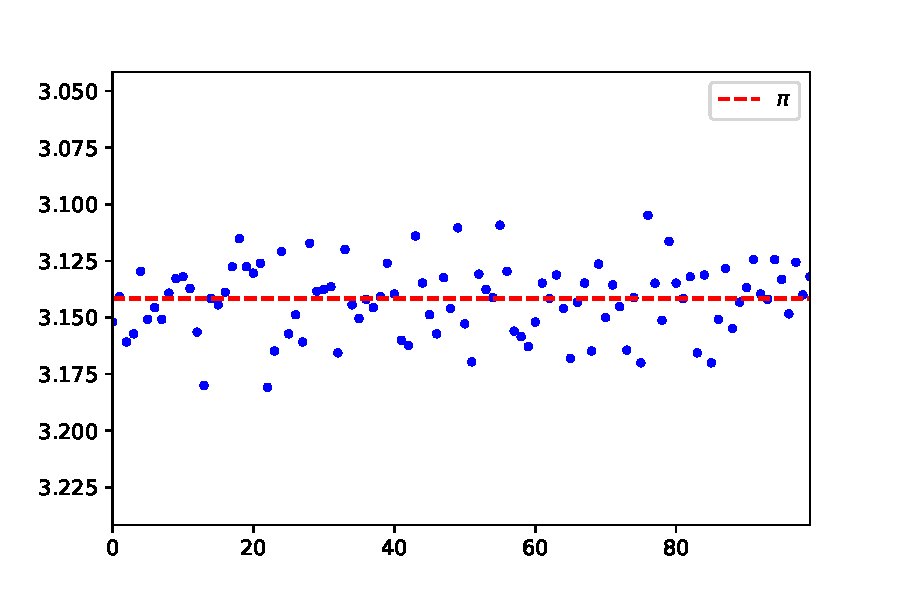
\includegraphics[width=0.7\textwidth]{images/variation.pdf}
\caption{Monte Carlo法求圆周率, 每次10000次随机投点,重复了100组。}
\label{fig::variation}
\end{figure}

增加投点数量显然可以减少模拟结果的波动,或者说,从随机算法的角度,提高
结果的精度。从图 \ref{fig::number2variation}可以看到,随着投点的增加,
模拟结果越来越聚集到精确$\pi$值的附近。这张图也很形象的表现了什么叫依
概率收敛。

\begin{figure}[!ht]
\centering
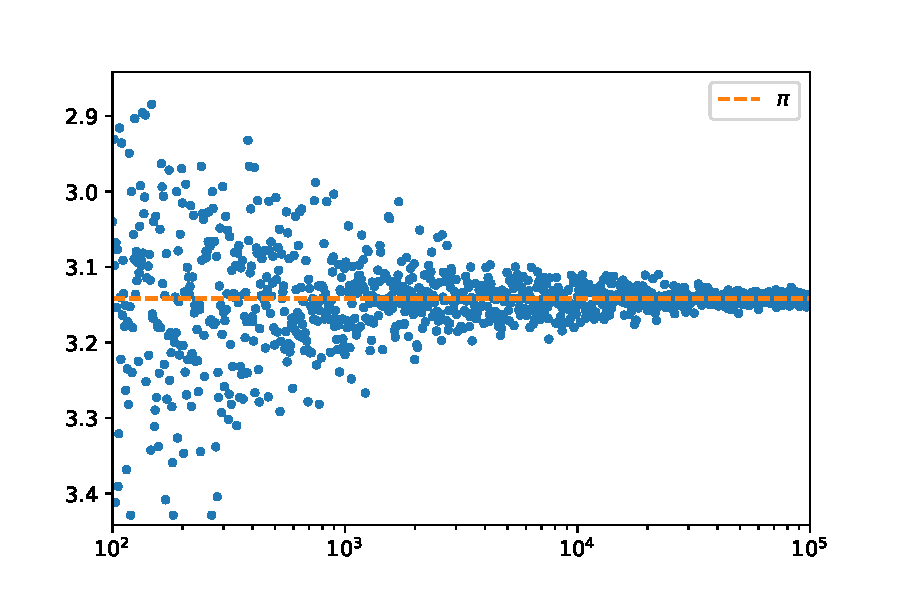
\includegraphics[width=0.7\textwidth]{images/number2variation.pdf}
\caption{Monte Carlo法求圆周率, 投点数从$10^2$到$10^5$, 按$\log$分布
  做了1000组。}
\label{fig::number2variation}
\end{figure}

Monte Carlo方法的优点和缺点都一样明显。好处是它只基于随机投点,整个过
程非常简单机械,非常适合计算机完成。在很多数学上根本无法建模的问题中,
它也能很好地实现。它确实是一种``万能''的方法。坏处就是,我们稍微思考一
下就能明白,它有效完全依赖于大数定律和中心极限定理。即随着独立试验的增
加,均值总是会依概率收敛到(设计好的)期望。那么误差在这里就会收敛到方
差!显然,误差是$\mathrm{O}(1 / \sqrt{n})$的(后续课程我们会精确分析这
  一过程)。这意味这如果我们在十进制下要增加一位有效数字,那么工作量会
增加100倍。而一般的数值积分方法,误差一般都是$\mathrm{O}(1 / n^p), p >
1$阶的。所以只有在相对复杂,经典数值方法无法给出高效算法的情况下,我们
才会考虑Monte Carlo方法。比如,极高维度的数值积分。我们注意到,经典数
值积分方法是维数相关的,随着空间维数的增加,为了得到同样阶精度,积分点
的数量也要以空间指数增加。比如在3维要达到$\mathrm{O}(1 / n^p), p > 1$
的精度,相对1维来说,积分点也要从$n$个增加到$\mathrm{O}(n^3)$个。于是
对于一些超高维数问题,经典数值方法变得非常昂贵。然而,大家也许已经注意
到,Monte Carlo方法是维数无关的,不管这个区域是几维,我们要做的就是随
机投点,数数。当然,实际上产生一个$m$维空间的随机点,相比1维空间,工作
量是其$m$倍。但至少只是一个线性增长。因此维数越高,Monte Carlo方法的优
势越明显。

\section{本课程内容}
在这个学期,我们的重点既不在概率论,也不在统计,甚至也不会专门讲太多的
计算机编程。(当然概率论是一切的理论基础,所以如果你没有学过概率论,那
  么赶紧去自学一下也许还能活。)我们将注意力更多的集中在随机算法和相应
的技术实现上。这其实是一门优化或者数学规划(Operations Research)的分支
课程。它变得如此重要的原因相信大家都是理解的。在目前大数据和AI领域的最
前沿,随机优化算法正在发挥巨大的作用。然而在传统的授课体系中,不论在计
算机学院还是数学院,和随机优化有关的内容之前都不是很受重视,至少缺乏系
统性的讲述。本课程的设计初衷就是试图弥补这个空缺。在接下去的一个学期中,
我们将从随机数的产生和随机抽样开始,逐步讨论Monte Carlo方法、模拟退火
算法、遗传算法等经典的随机优化方法,介绍它们的原理和实现。同时我们也会
重点分析一些比较重要的具体算法,比如神经网络中经常采用的随机梯度下降算
法。此外,我们也会解析几个重要案例,来体会这些理论和技术是如何具体问题
中得到应用。

由于这是一门面向全新领域的全新课程,所以以上的一切都还不是定案。在学习
过程中,我们可能随时根据需要增删。同时可能也会有大量的参考材料和技术资
料需要课外阅读。希望通过我们这一学期的努力,能够初步建立起这样一门关键
课程的框架和雏形。在这个过程中,需要我们每一位参与者的共同努力。


\chapter{随机数的产生}

随机模拟的关键是高质量的随机数。但计算机是一个确定性主导的系统。它无法
产生真正的随机数。因此,我们要么专门构建特殊的装置来产生真随机数,要么
通过一些数学公式来产生性质接近真随机数的伪随机数\cite{Kang2015MonteCarlo}。

\section{真随机数产生器}

真随机数产生器是一种物理装置,它依赖客观世界中的真实随机现象如基本粒子
的随机热运动,量子效应等来产生随机数。这种装置能产生几乎完美的随机数,
但往往产生效率不高,且装置本身较为昂贵。一种可以考虑的方法是使用真随机
数产生器生成的随机数表。比如网站:\\
\href{https://www.random.org}{https://www.random.org} \\
就提供这样的服务。
表\ref{table::random_org}是它的一张价格表。

\begin{table}
  \centering
  \begin{tabular}[!ht]{lll}
    \multicolumn{3}{l}{\bf Integers}\\
    \multicolumn{3}{l}{\bf Prices of Example Files}\\
    \hline
    \hline
Integers & Size of Range  & Price \\
\hline
50,000	& 10	& \$5.00 \\
\hline
250,000	& 1,000	& \$5.00 \\
\hline
1,000,000 & 100	& \$6.66 \\
\hline
5,000,000 & 1,000 & \$36.17 \\
\hline
10,000,000 & 1,000 & \$61.09\\
\hline
\end{tabular}
  \caption{网站 \href{https://www.random.org}{https://www.random.org}
    提供的随机整数表的价格。}
  \label{table::random_org}
\end{table}

随着伪随机数理论和实际质量的提高,以及真随机数在巨型计算系统上的应用限
制,如Monte Carlo法这样随机算法已经没有必要再使用真随机数,高质量的伪
随机数生成算法完全可以胜任。在继续讨论之前,我们先给出随机数的定义。

\begin{definition} {\hei 随机数} 从均匀分布$U(0, 1)$抽样得到的简单子样称为随机数,
  其概率密度函数为
  $$
  f(x) = 1, 0 \leq x \leq 1.
  $$
  随机数用专门符号$U$表示,序列$\{U_1, U_2, \cdots\}$代表独立同分布
  的随机序列。
  \label{def::psudo_random_number}
\end{definition}

随机数的一个非常重要的性质是高维分布均匀性。由$s$个随机数所组成的$s$维
空间上的点
$$
(U_{n + 1}, U_{n + 2}, \cdots, U_{n + s})
$$在$s$维空间的单位正方体$C_s$上是均匀分布的,即$\forall 0 \leq a_i
\leq 1$,$i = 1, 2, \cdots, s$,$U_{n + i} \leq a_i$的概率为:
\begin{equation}
  P(U_{n + i} \leq a_i, i = 1, 2, \cdots, s) = \prod_{i = 1}^s a_i.
\end{equation}

用数学方法产生的随机数称为伪随机数。Tezuka 1995 \cite{Shu1995Uniform}
提出伪随机数应该具有如下特点:
\begin{enumerate}
  \item 能通过统计检验;
  \item 有数学理论支撑;
  \item 可以递推产生,不用占用大量内存;
  \item 产生速度快,效率高;
  \item 重复周期长,至少有$10^{50}$;如果问题需要$N$个随机数,则周期需
    要$2N^2$;
  \item 并行性好,可在计算集群上快速产生;
\end{enumerate}

\section{早期伪随机数算法}

\subsection{经典Fibonacci产生器}

Taussky和Todd 1956年\cite{TausskyGeneration}提出可以用加法同余产生在
$[0, M-1]$均匀分布的伪随机整数,其递推公式为
\begin{equation}
  X_i = (X_{i - 2} + X_{i - 1})\mod M, i > 2.
  \label{eq::add_mod}
\end{equation}
当$X_0 = X_1 = 1$时,公式(\ref{eq::add_mod})产生的序列在小于$M$部分就是
Fibonacci序列,因此又称为经典Fibonacci产生器。该算法过程实现很简单。算
法\ref{alg::add_mod}给出了它的程序。显然,$U_i = X_i / M$给出了相应的
$U(0, 1)$分布随机数。

\begin{minipage}[!ht]{0.8\textwidth}
\vspace{3ex}
\refstepcounter{alg}
\label{alg::add_mod}
\begin{center}
 算法 \arabic{chapter}.\arabic{alg} 加法同余产生器
\end{center}
\small
\begin{tabular}{lll}
  \hei 输入&X0,X1&初值\\
  &M&最大整数值\\
  &N&随机数个数\\
  \hei 输出&&N个服从$U(0, 1)$分布的随机浮点数序列
\end{tabular}
\begin{lstlisting}[style = python]
def rand_add_mod(X0, X1, M, N):
    X = np.zeros(N)
    X[0] = X0
    X[1] = X1
    for i in range(2, N):
        X[i] = (X[i - 2] + X[i - 1]) % M
    return X / (M - 1)
\end{lstlisting}
\end{minipage}

尽管在简单的测试中,这个方案给出的伪随机数似乎还不错,比如图
\ref{fig::add_mod_random_test}中,我们看到在该序列的投点似乎非常均匀。
然而,在特殊的抽样公式
\begin{eqnarray}
  X_i & = & \sqrt{U_i} \cos(2 \pi U_{i + 1}) \sin(\pi U_{i + 2})
  \label{eq::add_mod_random_fail_x}\\
  Y_i & = & \sqrt{U_i} \sin(2 \pi U_{i + 1}) \sin(\pi U_{i + 2})
  \label{eq::add_mod_random_fail_y}
\end{eqnarray}
下,我们看到$X_i$和$Y_i$与应有的统计预测不符。见图
\ref{fig::add_mod_random_fail}。这说明,抽样公式
(\ref{eq::add_mod_random_fail_x})和(\ref{eq::add_mod_random_fail_y})实
际上回归出了加法同余产生器的规律。这在实际模拟中是非常危险的。除此以外,
文献指出,该算法还有其他较为严重的问题,比如随机序列不能居中$(U_i,
U_{i + 1}, U_{i + 2})$在3维空间分布相关等等。但同余运算在伪随机数生成
算法中,仍具有一定的意义。不少现在仍在使用的方法,是经典Fabonacci方法
的一个改进。

\begin{figure}[!ht]
\centering
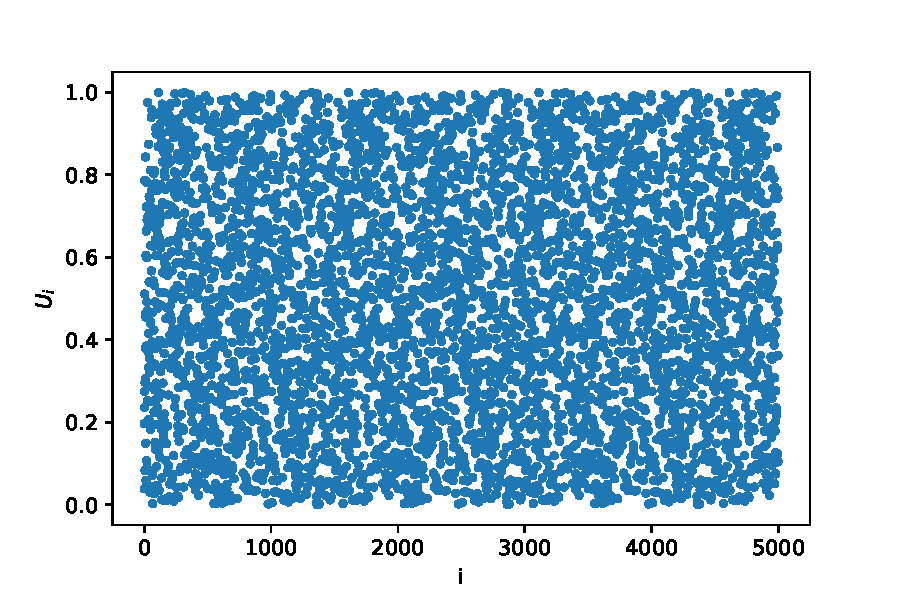
\includegraphics[width=0.7\textwidth]{images/add_mod_random_test.pdf}
\caption{加法同余产生器的均匀性测试, $X_0 = 197$,$X_1 = 39$, $M =
  1000$,一共产生了5000个随机数。}
\label{fig::add_mod_random_test}
\end{figure}

\begin{figure}[!ht]
\centering
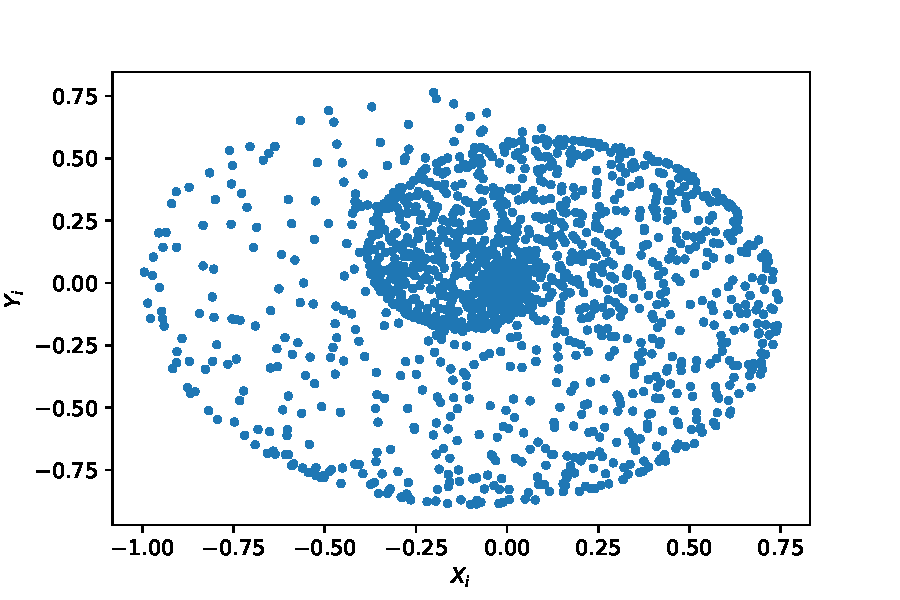
\includegraphics[width=0.7\textwidth]{images/add_mod_random_fail.pdf}
\caption{加法同余产生器的缺陷。在特殊抽样下与统计预测不符。$X_i$和
  $Y_i$分别用公式(\ref{eq::add_mod_random_fail_x})和
  (\ref{eq::add_mod_random_fail_y})产生。}
\label{fig::add_mod_random_fail}
\end{figure}

\subsection{线性同余产生器}

Lehmer 1951\cite{Lehmer1949Mathematical}和Rotenberg
1960\cite{Rotenberg1960A}分别提出了乘同余和混合同余产生器。递推公式为:
\begin{equation}
  X_i = (A * X_{i - 1} + C) \mod M,
  \label{eq::mul_mod}
\end{equation}
其中参数$M$,$A$和$C$分别称为模,乘子和增量。当$C = 0$的特例即是乘同余
产生器,而$C > 0$则称为混合同余产生器。同样可以用$U_i = X_i / M$将其调
整为$U(0, 1)$分布。算法\ref{alg::mul_mod}给出了具体的产生程序。

\begin{minipage}[!ht]{0.8\textwidth}
\vspace{3ex}
\refstepcounter{alg}
\label{alg::mul_mod}
\begin{center}
 算法 \arabic{chapter}.\arabic{alg} 混合同余产生器
\end{center}
\small
\begin{tabular}{lll}
  \hei 输入&X0&初值\\
  &M&最大整数值\\
  &A,C&人工参数\\
  &N&随机数个数\\
  \hei 输出&&N个服从$U(0, 1)$分布的随机浮点数序列
\end{tabular}
\begin{lstlisting}[style = python]
def rand_mul_mod(X0, M, A, C, N):
    X = np.zeros(N)
    X[0] = X0
    for i in range(1, N):
        X[i] = (A * X[i - 1] + C) % M
    return X / (M - 1)
\end{lstlisting}
\end{minipage}

不恰当地选择参数也会有有类似加同余的异常相关现象,
图\ref{fig::mul_mod_random_fail} 对参数$A = 7$,$M = 2^{31} - 1$给出在
特殊抽样
\begin{eqnarray}
  X_i & = & \sqrt{-2 \ln U_i} \cos(2 \pi U_{i + 1}) 
  \label{eq::mul_mod_random_fail_x}\\
  Y_i & = & \sqrt{-2 \ln U_i} \sin(2 \pi U_{i + 1}) 
  \label{eq::mul_mod_random_fail_y}
\end{eqnarray}
下的二维分布图。可以看到样本点全部落在一条螺旋线上。

\begin{figure}[!ht]
\centering
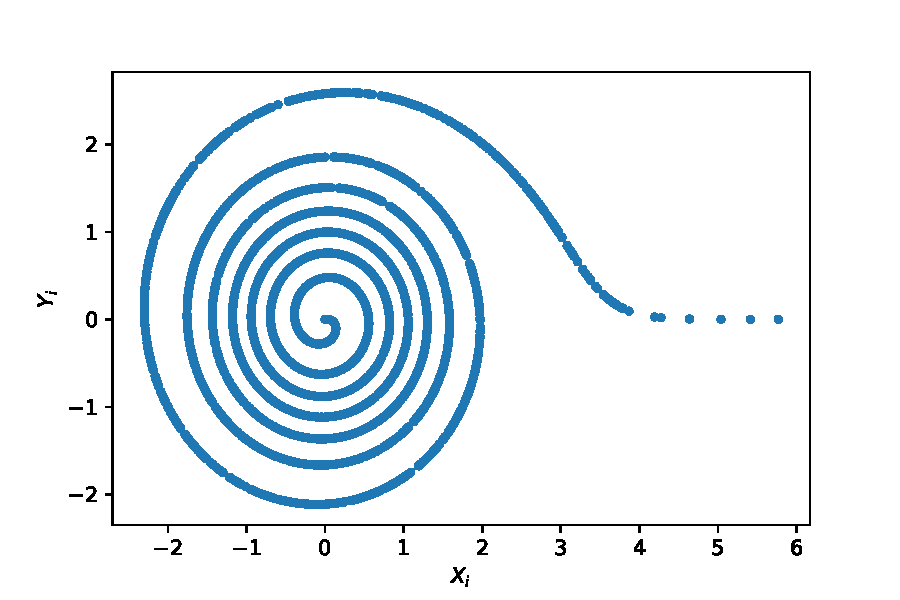
\includegraphics[width=0.7\textwidth]{images/mul_mod_random_fail.pdf}
\caption{线性同余产生器的缺陷。$X_i$和$Y_i$分别用公式
  (\ref{eq::mul_mod_random_fail_x})和(\ref{eq::mul_mod_random_fail_y})
  产生。所有的点都落在一条螺旋线上。}
\label{fig::mul_mod_random_fail}
\end{figure}

线性同余产生器的参数选择需要一些数论的概念。首先引入定义:

\begin{definition} {\hei 原根(Primitive Root)}
  称线性同余产生器参数乘子$A$是模$M$的原根,当且仅当
  \begin{enumerate}
    \item 
      \begin{equation}
        (A^{M - 1} - 1) \mod M  = 0;
        \label{eq::primitive_root}
      \end{equation}
    \item 任取$I < M - 1$, $(A^I - 1) / M$不是整数.
  \end{enumerate}
  \label{def::primitive_root}
\end{definition}

我们总是希望伪随机数的周期尽可能长(伪随机数周期总是会有的),在
\cite{Fishman1995Monte}中,作者指出当模$M$是素数时,当且仅当乘子$A$是
其原根时,乘同余产生器的周期是$M - 1$。因此我们一般将$M$取成$2^\beta -
1$(梅森数),这里$\beta$是机器字长。而对于混合同余产生器,模$M$一般取
$2^\beta$,其周期为$M$当且进当$A = 4k + 1$,$k \in \mathbb{N}$,且$M$
和$C$互质。

线性同余方法曾经广泛使用于各个计算机平台做为伪随机数发生器。比如IBM
360系统下曾有一个著名的随机数产生器RANDU被使用多年。它就是$A = 65539$,
$M = 2^{31}$的线性乘同余产生器。然而,可以验证,它的三重分布,即
$(U_{i}, U_{i + 1}, U_{i + 2})$只分布在15个空间平面上见图
\ref{fig::RANDU_fail},它们是:
\begin{equation}
  9x - 6y + z = k, k = -5, -4, \cdots, 8, 9.
\label{eq::RANDU_plain}  
\end{equation}
这一现象被称为降维,它导致随机数的高维分布均匀性消失。具体推导可参见:\\
\href{https://en.wikipedia.org/wiki/RANDU}{https://en.wikipedia.org/wiki/RANDU} \\

\begin{figure}[!ht]
\centering
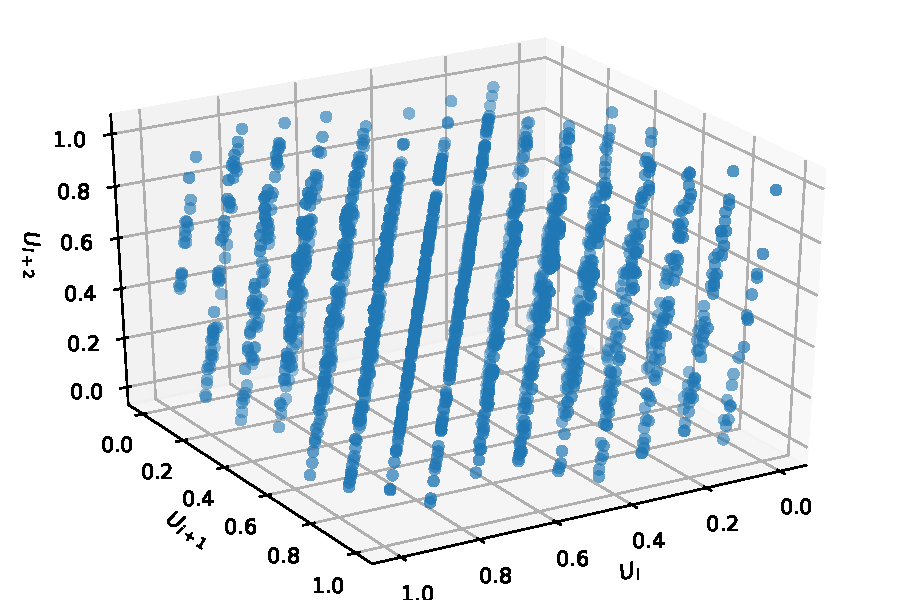
\includegraphics[width=0.7\textwidth]{images/RANDU_fail.pdf}
\caption{IBM360/370 RANDU的三维分布稀疏栅格现象。这里$A = 65539$,$M =
  2^{31}$,$C = 0$。}
\label{fig::RANDU_fail}
\end{figure}

可以证明,降维现象是线性同余产生器的一个必然结果。一般地,对与线性同余
产生器产生的伪随机点列构成的$s$维空间点列
\begin{equation}
  P = (U_i, U_{i + 1}, \cdots, U_{i + s - 1}), i = 1, 2, \cdots
  \label{eq::mul_mod_mul_dim_fail}
\end{equation}
只落在个数不超过$(s!M)^{1/s}$的彼此平行的超平面上(参见:
  \cite{Marsaglia1968Random})。

由于以上这些缺陷,目前的主流意见是不要单独使用线性同余产生器。特别是在
进行类似Monte Carlo模拟时,要格外警惕伪随机数的降维和异常相关现象。当
我们在具体的系统上运算时,也应该先阅读文档,查找具体的随机数产生方式。
比如,某些低版本的GCC编译器提供的伪随机数就有可能是$M = 2^{32}$,$A =
1103515245$,$C = 12345$的一个混合同余产生器。

\section{伪随机数产生器的进展}

线性同余算法尽管快速简单,但由于它的缺陷,人们陆续提出了一些新的算法以
产生更高质量的随机数。主要的改进思路来自以下几个方向:

\subsection{非线性同余产生器}
这种生成器的思想是当$M$是素数时,通过构建某种排列多项式,将$\{0, 1,
\cdots, M -1\}$作为一个Galois域重排成$\{g(0), g(1), \cdots, g(M -
1)\}$,然后在此基础上构建递推生成器。以继承这种基于重排的均匀性。

比如逆同余产生器:
\begin{equation}
  X_i = (A X_{i - 1}^{-1} + C) \mod M, i \geq 1.
  \label{eq::inv_lin}
\end{equation}
这里的$g(x) = x^{-1}$是一种非线性整函数,定义为:

\begin{definition} {\hei 乘法逆(multiplicative inverse)}
  称$z^{-1}$是$z$关于$M$的乘法逆,如果
  \begin{equation}
    z \cdot z^{-1} \mod M = 1, z^{-1} \in \mathbb{N}, z^{-1} < M.
    \label{eq::mul_inv}
  \end{equation}
  \label{def::mul_inv}
\end{definition}
并且规定$0$的乘法逆为$0$。

可以验证,对$M = 11$,$A = 8$,$C = 1$和$X_0 = 0$产生的前9个数是
$$
0, 1, 9, 8, 2, 5, 7, 10, 4, 3,
$$基本上就是$0 \sim 10$的重排(漏掉了6以外)。这种产生器可以通过很高维
的栅格检验,但是它的生成效率远低于线性同余。关于如何高效求乘法逆涉及数
论、群论和计算机算法的高深内容,有兴趣的同学可参见
\cite{Lidl1986Introduction}.

此外,常用的非线性同余产生器还有二次或高次同余,二次同余递推公式为:
\begin{equation}
  X_i = (A X_{i - 1}^2 + B X_{i - 1} + C) \mod M.
  \label{eq::q_mod}
\end{equation}
更多的内容可自行参考\cite{Fishman1995Monte, Kang2015MonteCarlo}。

\subsection{多步线性递推产生器}
即增加线性递推的递推层数,一般性的多步线性递推公式为:
\begin{equation}
  X_i = (A_1 X_{i - 1} + A_2 X_{i - 2} + \cdots + A_j X_{i - j}) \mod
  M, i \geq j.
  \label{eq::mul_lin}
\end{equation}
为提高效率,一般我们只保留其中两个系数$A_j$和$A_l$不为零,由此产生了一
系列具体的方案:

\begin{enumerate}
\item FMRG($A_1 = 1$,$A_l = B$),
  \begin{equation}
    X_i = (X_{i - 1} + B X_{i - l}) \mod M;
    \label{eq::fmrg}
  \end{equation}
\item DX-k-2($A_1 = A_l = B$),
  \begin{equation}
    X_i = B(X_{i - 1} + X_{i - l}) \mod M;
    \label{eq::dxk2}
  \end{equation}
\item DX-k-3($A_1 = A_{[l / 2]} = A_l = B$),
  \begin{equation}
    X_i = B(X_{i - 1} + X_{i -[1 / 2]} + X_{i - l}) \mod M;
    \label{eq::dxk3}
  \end{equation}
\item DX-k-4($A_1 = A_{l / 3} = A_{[2l /3]} = A_l = B$),
  \begin{equation}
    X_i = B(X_{i - [l /3]} + X_{i - [2l /3]} + X_{i - l}) \mod M.
  \end{equation}
\end{enumerate}
以上,$i \geq l$。这一系列公式的极致是L. Y. Deng 等人2003年设计的
DX3803生成器,周期长达$2^{117923}$,而且在3803维空间内分布均匀。参见:
\cite{Deng2003A}。

除了上面的方案,常用的改良手段还有进位借位运算产生器\cite{Shu1993On},
延迟Fibonacci生成器\cite{Brent1992Uniform},线性同余组合产生器
\cite{L1991Structural, Rose2014KISS},混合组合产生器
\cite{Fischer1999Good, Marsaglia2004The, Marsaglia1990Toward}等等,限
于篇幅不一一叙述,有兴趣的同学请自行查阅文献。

\section{梅森旋转(Mersenne Twister)产生器}

最后我们介绍一种目前最广泛使用的随机数产生器——梅森旋转产生器。它基于四
位日本数学家所发表的一系列论文,Matsumoto(松本) \& Kurita(栗田)
1992, 1994\cite{Matsumoto1992Twisted, Matsumoto1994Twisted},Matsumoto
\& Nishimura(西村) 1998, 2000
\cite{Matsumoto2000Dynamic, Matsumoto1998Mersenne},Matsumoto \& Saito(斋藤)
2008\cite{Saito2008SIMD}。它的一个重要实例MT19937被几乎所有重要编程平
台包括并不限于:C,C++,Python,Matlab等所采纳。它周期长达$2^{19937}-1$,
能通过目前几乎所有的随机数检验程序,且在至多623维空间分布均匀。MT19937
是基于32位字长机器运算。下面我们来介绍MT19937的具体实现过程。本章代码在
cnblog上网友xlxw的blog《Python下探究随机数的产生原理和算法》,网址:\\
\href{https://www.cnblogs.com/lzxwalex/p/6880748.html}
     {https://www.cnblogs.com/lzxwalex/p/6880748.html} \\
提供的代码基础上修改而成,并参考了CSDN网友tick\_tokc97的blog
《伪随机数生成——梅森旋转(Mersenne Twister/MT)算法笔记》\\
\href{https://blog.csdn.net/tick_tock97/article/details/78657851}
     {https://blog.csdn.net/tick\_tock97/article/details/78657851}。


\subsection{初始化}
梅森旋转需要有一个工作区。MT19937的工作区是一个长度为624的数组,每个元
素都是32位字长的整数。生成工作区的过程称为初始化。初始化本身也是一个伪
随机数产生过程,这个过程采用了类似线性产生器,并混合了位运算以保证产生
数字在二进制位的形式上分布均匀。具体公式为:
\begin{equation}
  M_i = f * (M_{i - 1} \oplus (M_{i - 1} >> (w - 2))) + i, i = 1, 2, \cdots, 624.
  \label{eq::MT19937_init}
\end{equation}
这里32位整数向量$M$存放的就是工作区,$M_0$由用户作为种子给出,$f$是
参数,在MT19937中取1812433253(十六进制:6C078965)。运算符$\oplus$表
示异或运算XOR,$w$表示机器字长,在MT19937中取32。具体的算法代码见算法
\ref{alg::MT19937_init},

\begin{minipage}[!ht]{0.8\textwidth}
\vspace{3ex}
\refstepcounter{alg}
\label{alg::MT19937_init}
\begin{center}
 算法 \arabic{chapter}.\arabic{alg} MT19937工作区初始化
\end{center}
\small
\begin{tabular}{lll}
  \hei 输入&seed&随机数种子\\
  &M&存储梅森工作区的空间\\
  \hei 输出&&生成的梅森工作区
\end{tabular}
\begin{lstlisting}[style = python, escapechar = \%]
# 转换成32位整数。
def inter(t):
    return(0xFFFFFFFF & t) #截取最后32位

def mainset(seed, M):
    M[0] = seed    
    for i in range(1,624):
        M[i] = inter(1812433253 * (M[i - 1] ^ M[i - 1] >> 30) + i)
    return M
\end{lstlisting}
\end{minipage}

初始化本身就是一个还算不错的伪随机数产生器。

\subsection{梅森旋转}
接下去通过梅森旋转,直接从二进制层面在整个工作区重新分布0和1,并且用旋
转和异或操作使二进制数分布均匀。由于工作区的长度是624,故每产生624个数,
都要重新执行一次梅森旋转。
\begin{equation}
  M_i = M_{i + m} \oplus ((\mbox{upper\_mask}(M_i) ||
  \mbox{lower\_mask}(M_{i+1}))A)
  \label{eq::MT19937_twister}
\end{equation}
此处,$\mbox{upper\_mask}(M_i)$和$\mbox{lower\_mask}(M_{i + 1})$分别表
示取$M_i$和$M_{i + 1}$的高$w - r$位和低$r$(在MT19937中$w = 32$,$r =
  31$),符号$||$表示将两边的高位和低位连接成一个32位的数。下一步$xA$
运算的定义为:
\begin{equation}
  xA = \left\{
  \begin{array}{ll}
    x >> 1, & x_0 = 0, \\
    (x >> 1) \oplus a, & x_0 = 1.
  \end{array}
  \right.
\end{equation}
这里$x_0$表示$x$的最低位,$a$是给定参数,在MT19937中设置为
0x9908B0DF(十六进制)。最后将$i$后第$m$个工作区数(在MT19937中$m =
  397$),即$M_{i + m}$拿来和连接成的数做异或,注意上述下标$i + 1$和$i
+ m$在实际实现中都要和624取模,因此实际上整个工作区是循环边界的。这也
是梅森旋转的名字中旋转的来历。完整的算法过程见算法
\ref{alg::MT19937_twister}。

\begin{minipage}[!ht]{0.8\textwidth}
\vspace{3ex}
\refstepcounter{alg}
\label{alg::MT19937_twister}
\begin{center}
 算法 \arabic{chapter}.\arabic{alg} MT19937梅森旋转
\end{center}
\small
\begin{tabular}{lll}
  \hei 输入&梅森工作区的空间\\
  \hei 输出&旋转后的梅森工作区
\end{tabular}
\begin{lstlisting}[style = python]
def twister(M):
    for i in range(624):
        # 截取M[i]高位和M[i+1](越界就返回M[0])低位,用普通加法合并,对齐32位
        # 这里高位取了1位,低位取了31位。
        y = inter((M[i] & 0x80000000) +(M[(i + 1) % 624] & 0x7fffffff))
        yA = y >> 1
        if y & 1 == 1: #取最低位
            yA = yA ^ 0x9908b0df
        M[i] = M[(i + 397) % 624] ^ yA
    return M
\end{lstlisting}
\end{minipage}

\subsection{递推}
最后我们可以利用工作区,产生梅森旋转的递推公式:
\begin{eqnarray}
  y &=& x \oplus ((x >> u) \& d),\\
  \label{eq::MT19937_recursion1}
  y &=& y \oplus ((y << s) \& b),\\
  \label{eq::MT19937_recursion2}
  y &=& y \oplus ((y << t) \& c), \\
  \label{eq::MT19937_recursion3}
  z &=& y \oplus (y >> l). 
  \label{eq::MT19937_recursion4}
\end{eqnarray}
这里$x$依次从$M$中取,取完624个则重新执行梅森旋转。$y$是中间变量,$z$
是返回的下一个随机数。其他$u$,$d$,$s$,$b$,$t$,$c$和$l$均为人工参数。在
MT19937中,$l = 18$,其余参数分别取作
\begin{eqnarray*}
  (u, d) &=& (11, \mbox{0xFFFFFFFF$_{16}$}),\\
  (s, b) &=& (7, \mbox{0x9D2C5680$_{16}$}),\\
  (t, c) &=& (15, \mbox{0xEFC60000$_{16}$}), \\
\end{eqnarray*}
这里第二列都是十六进制。

最后,完整的随机数生成算法见\ref{alg::MT19937}。

\begin{minipage}[!ht]{0.8\textwidth}
\vspace{3ex}
\refstepcounter{alg}
\label{alg::MT19937}
\begin{center}
 算法 \arabic{chapter}.\arabic{alg} MT19937主流程
\end{center}
\small
\begin{tabular}{lll}
  \hei 输入&seed&随机数种子\\
  &num&随机数个数\\
  \hei 输出&&num个服从$U(0, 1)$分布的随机浮点数序列
\end{tabular}
\begin{lstlisting}[style = python]
def exnum(M, index):
    y = M[index]
    y = y ^ y >> 11
    y = y ^ y << 7 & 2636928640
    y = y ^ y << 15 & 4022730752
    y = y ^ y >> 18
    index = index + 1
    return inter(y)
    
def MT19937(seed, num):
    U = [0]*num
    M = [0]*624
    M = mainset(seed, M)
    twister(M)
    for i in range(num):
        index = i % 624
        U[i] = exnum(M, index) / (2**32 - 1)
        if (index == 623):
            twister(M)
    return U     
\end{lstlisting}
\end{minipage}

由于梅森旋转当中大量核心算法是位运算,因此运算效率极高,且便于机器底层
实现。这也是它成为目前最通用和最受欢迎的伪随机数生成算法。它同样也有64
和128位版本。其作者还在不断提高其计算效率和随机数质量,最新的进展可参
见广岛大学提供的网站:\\
\href{http://www.math.sci.hiroshima-u.ac.jp/~m-mat/MT/emt.html}
     {http://www.math.sci.hiroshima-u.ac.jp/~m-mat/MT/emt.html}。

\section{多维随机数产生方法}
多维随机数有直接产生的方法,具体参见Niederreiter
1992\cite{Niederreiter1992Random},这种方法产生的多维随机数性质较好,
但更为简便的方法是基于下述概率论定理用一维随机数间接产生:

\begin{theorem}
  若$\{A_i, i = 1, 2, \cdots, ns\}$是独立同分布的随机变量序列,
  则
  \begin{equation}
    \{(A_{(i - 1)s + 1}, A_{(i - 1)s + 2}, \cdots, A_{is}), i = 1, 2, \cdots\}
    \label{thm::mulvar}
  \end{equation}
  必是$s$维独立同分布的随机向量序列。而且每个分量序列
  \begin{equation}
    \begin{array}{rcl}
      \mathrm{U}_1 &=& \{U_1, U_{s + 1}, \cdots, U_{(n - 1)s + 1}\},\\
      \mathrm{U}_2 &=& \{U_2, U_{s + 2}, \cdots, U_{(n - 1)s + 2}\},\\
      &\cdots&\\
      \mathrm{U}_s &=& \{U_s, U_{2s}, \cdots, U_{ns}\},
    \end{array}
  \end{equation}
  在各自的维度中也是独立同分布的。
\end{theorem}

我们用上面的MT19937产生一维50万个随机数,并按定理次序重新组织成500个
1000维的随机向量。观察一下$(U_1, U_2)$和$(U_{999}, U_{1000})$平面的随
机数分布,都很均匀(见图\ref{fig::MT19937_1000D})。

\begin{figure}[!ht]
\centering
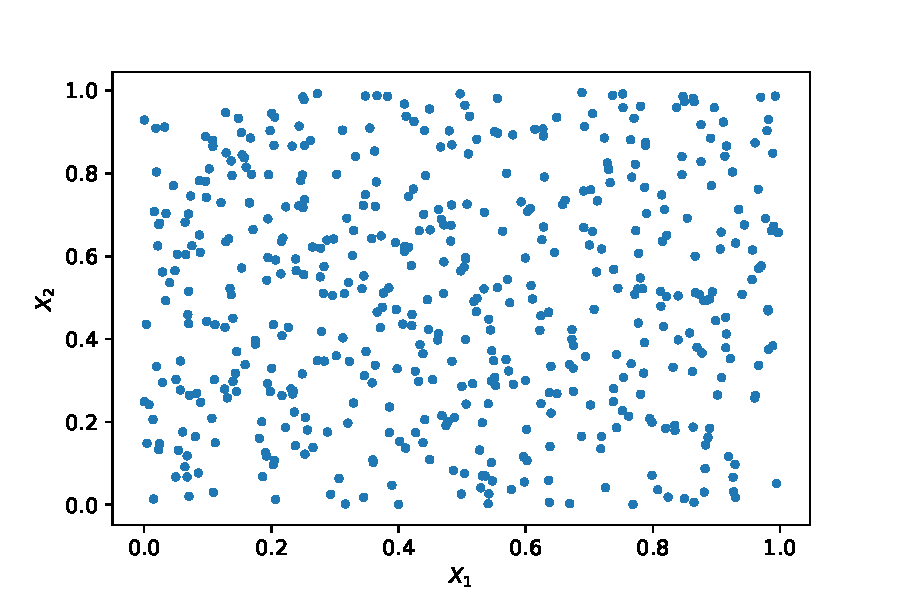
\includegraphics[width=0.45\textwidth]{images/MT19937_X1X2.pdf}
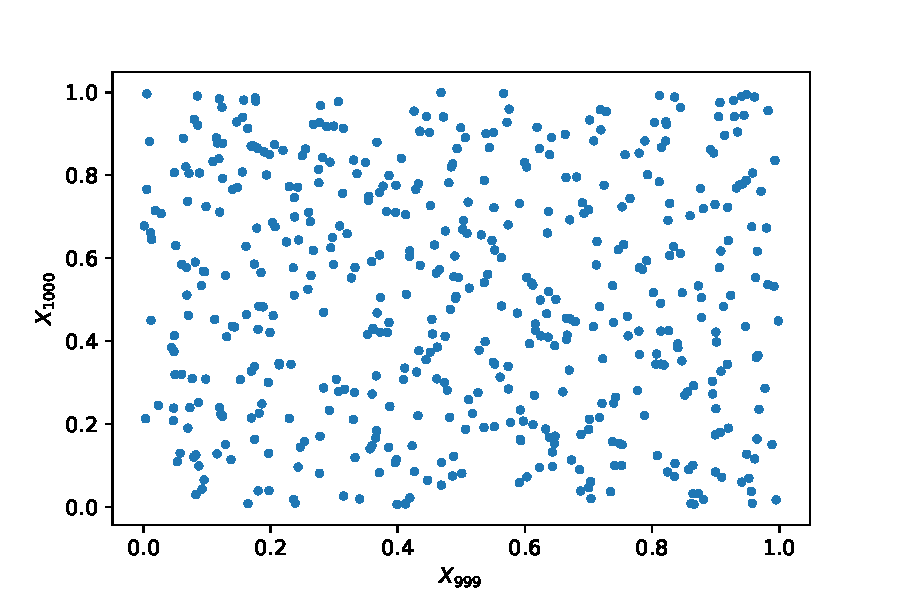
\includegraphics[width=0.45\textwidth]{images/MT19937_X999X1000.pdf}
\caption{用MT19937生成50万个随机数,重新组织成500个1000维随机向量。左
  图和右图分别是第$(1, 2)$维和第$(999, 1000)$维平面的随机数分布情况。}
\label{fig::MT19937_1000D}
\end{figure}

\section{随机数的检测}

随机数的理论检测即从随机数的产生原理出发,寻找它的缺陷。比如之前的栅格
现象(图\ref{fig::RANDU_fail})等。实际上这种缺陷也是在应用过程中发现,
才被人们所重视,并且在设计随机数产生器时格外注意。理论检验都只针对具体
的产生原理,并没有一般性。更多的,我们需要用现代统计学手段对随机数的质
量进行统计分析。较为一般的检验,可以是检查随机数的频率,频次,相关性,
各阶矩等等。更复杂的检验,则要精确设计统计实验,并涉及到较为复杂和专业
的统计学知识。目前被大家所接受的统计学检验程序是Marsaglia给出的DieHard
程序。它由一系列精心设计的复杂统计实验组成,几乎是目前检测随机数质量的
标准过程。George Marsaglia教授已于2011年去世,但DieHard程序仍然有人不
断更新和维护,并引入了GPL协议使得可以公开下载和免费使用。具体可参见网
站:\\
\href{http://webhome.phy.duke.edu/\~rgb/General/dieharder.php}
     {http://webhome.phy.duke.edu/~rgb/General/dieharder.php}
     \\

     


\chapter{随机抽样}

上一章我们讨论了最简单的随机分布,均匀分布随机数的产生方法。有了这个均
匀分布随机数的基础,这一章我们将进一步讨论如何产生各种所需的随机变量和
随机过程。首先我们回顾一下概率论的一些基本定义。

\section{基础知识回顾}
我们用概率分布来描述一个随机变量服从的分布规律,具体来说,离散型随机变
量的概率分布称为

\begin{definition} {\hei 概率质量函数(Probability Mass Function, PMF)}
  若离散型随机变量$\xi$取值为$x_1, x_2, \cdots, x_n$的概率分别为$p_1,
  p_2, \cdots, p_n$, 即
  \begin{equation}
    P(\xi = x_i) = p_i, i = 1, 2, \cdots, n,
    \label{eq::dis_df}
  \end{equation}
  则其概率分布函数
  \begin{equation}
    f(x) = \left\{
    \begin{array}{ll}
      p_i, & x \in S,\\
      0, & x \in \mathbb{R}\setminus S
    \end{array}\right.
    \label{eq::dis_pmf}
  \end{equation}
  又称为概率质量函数,简称为PMF。其中$S = \{x_1, x_2, \cdots, x_n\}$称
  为样本集。显然,在离散的情形下,有
$$
\sum_{x_i \in S}p_i = \sum_{i = 1}^np_i = 1.
$$
\label{def::dis_pmf}
\end{definition}


\begin{definition} {\hei 累积分布函数(Cumulative Distribution Function, CDF)}
  称
  \begin{equation}
    F(x) = P(\xi \leq x) = \sum_{x_i \leq x}p_i, x \in \mathbb{R}
    \label{eq::dis_cdf}
  \end{equation}
  为累积分布函数,简称为CDF。
  \label{def::dis_cdf}
\end{definition}

\begin{example} {\hei 两点分布} 最简单的两点分布的PMF为
  \begin{equation}
    f(x) = \left\{\begin{array}{ll}
    0.5, &x = 0; \\
    0.5, &x = 1;\\
    0, &x \notin \{0, 1\}.
    \end{array}\right.
    \label{eq::2p_PMF}
  \end{equation}
  对应的CDF为
  \begin{equation}
    F(x) = \left\{\begin{array}{ll}
    0, & x < 0; \\
    0.5, &0 \leq x < 1; \\
    1, &x = 1.
    \end{array}\right.
    \label{eq::2p_CDF}
  \end{equation}
  \label{example::2p}
\end{example}

更常见的,离散型随机变量的特征会像下面那样表示。

\begin{example} {\hei 二项分布} 的PMF一般写做
\begin{equation}
  b(k; n, p) = \binom{n}{k}p^k(1 - p)^{n - k}, 0 < p < 1, k = 0, 1, \cdots, n.
  \label{eq::binom_PMF}
\end{equation}
\label{example::binom}
\end{example}

我们考虑$n = 10$,$p = 0.3$的特例,我们可以根据其PMF给出对应的二项分布
表\ref{table::df_bin},以及对应的图\ref{fig::DF_bin}。

\begin{table}[!ht]
  \centering
  \caption{二项分布表,$n = 10$,$p = 0.3$}
  \label{table::df_bin}
\begin{tabular}{|c|c|c|c|}
  \hline
  $k$&0&1\\
  \hline
  $P(\xi = k)$&0.028247524900000005&0.12106082100000018\\
  \hline
  $k$&2&3\\
  \hline
  $P(\xi = k)$&0.2334744405&0.26682793200000016\\
  \hline
   $k$&4&5\\
   \hline
   $P(\xi = k)$&0.20012094900000013&0.10291934520000007\\
   \hline
   $k$&6&7\\
   \hline
   $P(\xi = k)$&0.03675690899999999&0.009001692000000002\\
   \hline
   $k$&8&9\\
   \hline
   $P(\xi = k)$&0.0014467004999999982&0.00013778100000000015\\
   \hline
   $k$&10&\\
   \hline
   $P(\xi = k)$&5.904899999999995e-06& \\
   \hline
\end{tabular}
\end{table}

\begin{figure}[!ht]
\centering
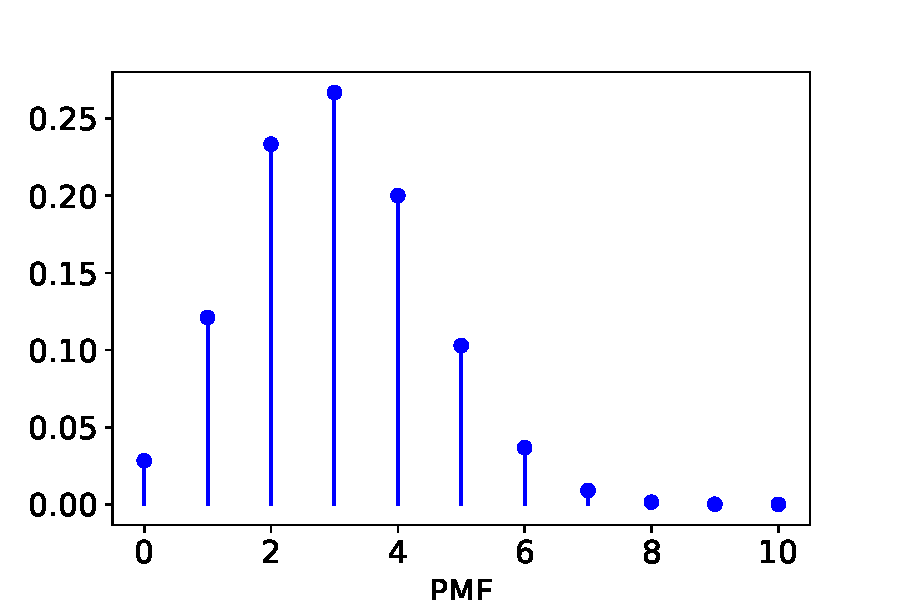
\includegraphics[width=0.45\textwidth]{images/PMF_bin.pdf}
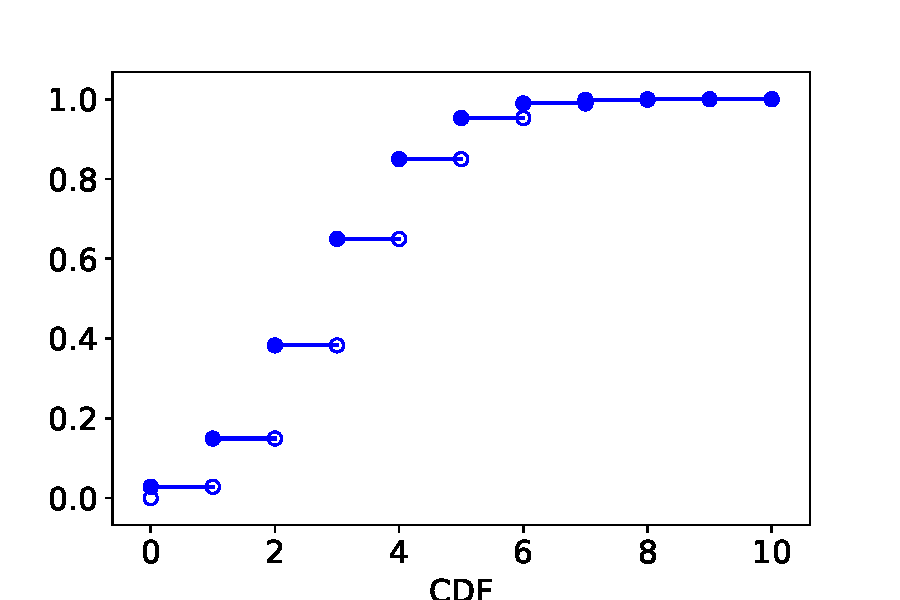
\includegraphics[width=0.45\textwidth]{images/CDF_bin.pdf}
\caption{二项分布,$n = 10$,$p = 0.3$,左:PMF,右:CDF。}
\label{fig::DF_bin}
\end{figure}

随机模拟的一个重要步骤是根据需要产生服从各种分布的样本集。之前我们已经
讨论过如何产生服从$U(0, 1)$的均匀分布的随机数,那么现在,我们就要从服
从$U(0, 1)$的均匀分布的随机序列出发,产生独立同分布的目标随机数序列。
这里两个问题的解决是各自独立的。首先随机序列的独立性完全由均匀分布的随
机序列的独立性决定,这在上一章已经讨论。我们接下去主要讨论如何确保随机
序列同分布,也即和要求的目标分布一致。这里还有一个重要问题是产生效率,
因为我们必须在计算机上算法实现。

\section{直接抽样方法}
如果随机变量的PMF是已知的,那么我们可以从均匀分布的随机数出发,直接根
据概率论定义构建抽样算法。这种方法称为直接抽样方法。即产生均匀分布的随
机序列,然后通过某种变换或抽取,使得从中变换抽取后的随机数样本集$X$服
从$F(x)$,这里$F(x)$是已知积累分布函数。也即要求$\forall \xi \sim F$,
\begin{equation}
  P(\xi \leq x) = F(x), x \in \mathbb{R}.
  \label{eq::def_cdf}
\end{equation}
这里,一方面,我们要从算法保证(证明)$X$确实服从指定分布$F(x)$;另
一方面,对于一个实际的产生的抽样结果,也要能通过指定的统计检验。

\subsection{逆变换算法}

1947年,曼哈顿计划的参与者Stanislaw Marein Ulam提出了逆变换算法,注意
到随机变量$\xi$的累积分布函数$F(x): \mathbb{R} \mapsto [0, 1]$是非降
的,故定义其逆函数为
\begin{equation}
  F^{-1}: [0, 1] \mapsto \mathbb{R}, F^{-1}(y) = \inf \{x \left| F(x)
  \geq y \right.\}
  \label{eq::inv_cdf}
\end{equation}

\begin{theorem}{}
  若随机变量$\eta$服从$[0, 1]$上的均匀分布,$F(x)$是指定分布的CDF,令
  $\xi = F^{-1}(\eta)$,则$\xi$服从$F(x)$.

  \noindent{\hei 证明:} $\forall x \in \mathbb{R}$,
  \begin{equation}
    P(\xi \leq x) = P(F^{-1}(\eta) \leq x) = P(\eta \leq F(x)) = F(x).
    \label{eq::prof_inv_cdf}
  \end{equation}
  证毕.
  \label{thm::inv_cdf}
\end{theorem}

所以我们算法的设计思路就是对一个均匀分布的随机数序列$U$,求其逆变换$X
= F^{-1}(U)$,则$X$的分布服从$F(x)$。

\subsection{列表查找法}
这种做法一般针对离散分布,特别是能给出分布表的离散分布。若离散分布的PMF表为
$$
\begin{array}{cccc}
  x_0 & x_1 & \cdots & x_n \\
  p_0 & p_1 & \cdots & p_n,
\end{array}
$$
且$x_0 < x_1 < \cdots < x_n$, 则我们不难构建CDF表
$$
\begin{array}{cccccc}
  x_0 & x_1 & \cdots & x_k & \cdots & x_n \\
  F_0 = p_0 & F_1 = p_0 +  p_1 & \cdots
  & F_k = \sum_{i = 0}^k p_i & \cdots & F_n \equiv 1.
\end{array}
$$
根据定义\ref{def::dis_pmf},$\forall x \notin \{x_0, x_1, \cdots,
x_n\}$,有$f(x) = 0$,故我们可以认为$F_{-1} = 0$。现在对$\eta \sim U(0, 1)$,
必有$0 \leq k \leq n$(为什么?), 满足
\begin{equation}
  \label{eq::def_dis_pmf}
F_{k - 1} < \eta \leq F_k,
\end{equation}
则可取$\xi = x_k$。从PMF角度,就是
\begin{equation}
  \xi = \min\left\{x_k\left|\eta \leq \sum_{i = 0}^kf(x_i)\right.\right\}, \eta \sim U(0, 1).
  \label{eq::dis_inv}
\end{equation}
在具体的抽取算法中,这一过程就是查表。对于较长的表,应该注意采用二分查
找(不知为何经典教材都是顺序遍历,大家仔细想想我有没有bug?)。具体算
法见算法\ref{alg::dis_sample_table}。

\begin{minipage}[!ht]{0.8\textwidth}
\vspace{3ex}
\refstepcounter{alg}
\label{alg::dis_sample_table}
\begin{center}
 算法 \arabic{chapter}.\arabic{alg} 离散随机分布的查表抽样
\end{center}
\small
\begin{tabular}{lll}
  \hei 输入&F&CDF\\
  &eta&$U(0,1)$分布的随机变量\\
  &start&起始抽样点\\
  &end&终止抽样点\\
  \hei 输出&&服从F分布的随机变量
\end{tabular}
\begin{lstlisting}[style = python]
def bisection_search(F, eta, start, end):
    if (eta <= F[start]):
        return start
    n = end - start
    if (n <= 0):
        sys.exit()
    k = (start + end) // 2
    if (eta > F[k]):
        if (eta <= F[k + 1]):
            return k + 1
        else:
            return bisection_search(F, eta, k + 1, end)
    else:
        return bisection_search(F, eta, start, k)
\end{lstlisting}
\end{minipage}

图\ref{fig::dis_bin_stat}给出了对$n = 10, p = 0.3$的二项分布的100万次抽样的统计检验结果。可以看到统计结果和理论PMF符合的很好。

\begin{figure}[!ht]
\centering
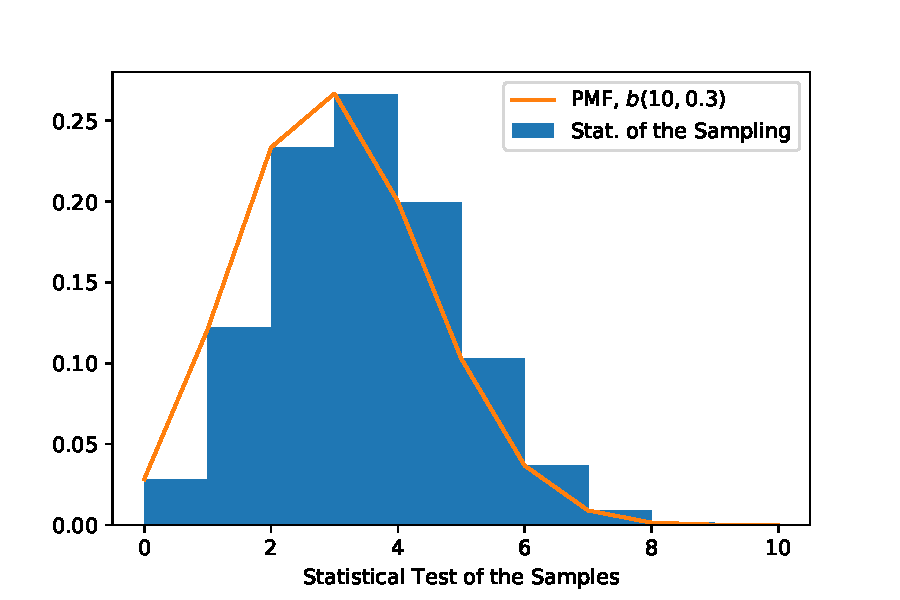
\includegraphics[width=0.7\textwidth]{images/test_bin.pdf}
\caption{对算法\ref{alg::dis_sample_table}抽样生成的$n = 10$,$p =
  0.3$二项分布的统计检验。柱状图是对100万次抽样生成样本集分布的统计,
  折线是$b(10, 0.3)$的PMF。二者吻合一致。}
\label{fig::dis_bin_stat}
\end{figure}


\subsection{连续分布的情形}
而对于连续型随机变量,可以看作是离散型随机变量的一种极限情形。此时概率
分布无法逐点定义,而是定义在样本集内的正测度集上,即考察随机变量落在一
个正测度集内的概率是多少。而从这个角度我们发现,之前在定义
\ref{def::dis_cdf}所引入的累积分布函数
$$
F(x) = P(\xi \leq x), x \in \mathbb{R}
$$
对连续型随机变量仍然适用,而在此基础上,可进一步引入直观上``概率如何
在一点上的定义''。由于一点是零测度集,所以这种定义无法脱离正测度集的概
念独立存在,而被看作``微元正测度集''的概率。

\begin{definition} {\hei 概率密度函数(Probability Density Function, PDF)}
  对连续型随机变量,$\forall x \in \mathbb{R}$, 我们仍称
  \begin{equation}
    F(x) = P(\xi \leq x), x \in \mathbb{R}
    \label{eq::df}
  \end{equation}
  为累计分布函数,若存在某个非负的可积函数$f(x)$,满足
  \begin{equation}
    F(x) = \int_{-\infty}^x f(y) dy, \forall x \in \mathbb{R},
    \label{eq::pdf}
  \end{equation}
  则称$f(x)$为对应随机分布的概率密度函数,简称为PDF。此时,
  \begin{equation}
    f(x) = F'(x).
    \label{eq::pdf2cdf}
  \end{equation}
  \label{def::pdf}
\end{definition}
注意到我们之前定义的针对离散型随机变量的PMF,事实上和这里定义的PDF
并无冲突,甚至可以看作是PDF的一个特例(这里要看你如何定义积分了)。关
于逆变换的定义也可以完全沿用。

\renewcommand\arraystretch{1.5}
\begin{table}[!ht]
  \centering
  \caption{常用连续概率分布的PDF和逆变换}
  \label{table::pdf_inv}
\begin{tabular}{|l|l|l|}
  \hline
  概率分布&PDF&逆变换\\
  \hline
  \small 均匀分布&$\frac{1}{b - a}, x \in [a, b]$&$a + (b - a)y$\\
  \hline
  \small Rayleigh分布&$\frac{x}{\sigma^2}e^{-\frac{x^2}{2\sigma^2}}, x > 0$
  &$\sqrt{-2\sigma^2\ln y}$\\
  \hline
  \small 指数分布&$\frac{1}{\lambda} e^{-\frac{x}{\lambda}}, \lambda > 0, x \geq 0$
  &$-\lambda\ln y$\\
  \hline
  \small Weibull分布&$\frac{a}{b^a}x^{a - 1} e^{-\left(\frac{x}{b}\right)^a},
  a, b > 0, x \geq 0$
  &$b\left(-\ln y\right)^{\frac{1}{a}}$\\
  \hline
  \small Beta分布&$ax^{a - 1}, a > 0, x \in [0, 1]$&$y^{\frac{1}{a}}$\\
  \hline
  \small Beta分布&$b(1 - x)^{b - 1}, b > 0, x \in [0, 1]$&$1 - y^{\frac{1}{b}}$\\
  \hline
  \small 逻辑分布&$\frac{e^{-\frac{x - a}{b}}}{b\left[1 + e^{-\frac{x - a}{b}}\right]^2}, b > 0$&$a + b \ln\left[\frac{y}{1 - y}\right]$\\
  \hline
  \small Cauchy分布&$\frac{b}{\pi\left[b^2 + (x - a)^2\right]}$
  &$a + \frac{b}{\tan(\pi y)}$\\
  \hline
  \small 正态分布&$\frac{1}{\sqrt{2\pi\sigma^2}}e^{-\frac{(x - \mu)^2}{2\sigma^2}}$&*\\
  \hline
  \small Pareto分布&$\frac{ab^a}{x^{a + 1}}, x \geq b > 0, a > 0$&$\frac{b}{(1 - y)^{\frac{1}{a}}}$\\
  \hline
\end{tabular}
\end{table}
\renewcommand\arraystretch{1}

对于连续分布的采样抽取,如果存在容易计算的逆变换解析表达式$F^{-1}(y)$,
那么对于$U(0, 1)$的均匀分布的随机变量$\eta$,直接计算$F^{-1}(\eta)$即
可。也就是说,
\begin{equation}
  \xi = \min\left\{x \left|\eta \leq \int_{-\infty}^x f(t)
  dt\right.\right\} = F^{-1}(\eta), \eta \sim U(0, 1),
  \label{eq::inv}
\end{equation}
则$\xi \sim f(x)$。算法\ref{alg::sample_inv_method}给出了Rayleigh分布
逆变换抽样的实现。

\begin{minipage}[!ht]{0.8\textwidth}
\vspace{3ex}
\refstepcounter{alg}
\label{alg::sample_inv_method}
\begin{center}
 算法 \arabic{chapter}.\arabic{alg} Rayleigh分布的逆变换抽样
\end{center}
\small
\begin{tabular}{lll}
  \hei 输入&U&$U(0, 1)$分布的随机序列\\
  &sigma&Rayleigh分布参数\\
  \hei 输出&&服从Rayleigh分布的浮点随机数组
\end{tabular}
\begin{lstlisting}[style = python]
def sample_Rayleigh(U, sigma):
    return [np.sqrt(-2 * sigma**2 * np.log(u)) for u in U]
\end{lstlisting}
\end{minipage}

\begin{figure}[!ht]
\centering
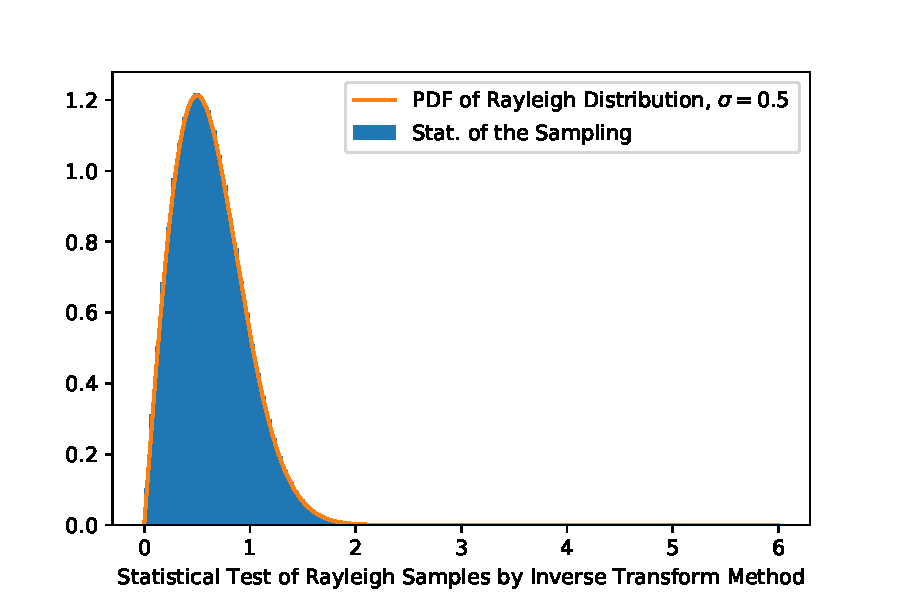
\includegraphics[width=0.7\textwidth]{images/Ray_inv.pdf}
\caption{对算法\ref{alg::sample_inv_method}抽样生成的Rayleigh分布
  ($\sigma = 0.5$)的统计检验。柱状图是对100万次抽样生成样本集分布的
  统计,折线是Rayleigh的PDF。二者吻合一致。}
\label{fig::Ray_stat}
\end{figure}

图\ref{fig::Ray_stat}给出了Rayleigh分布($\sigma = 0.5$)的采样结果和
PDF的对比。可以看到对于能快速计算逆变换的分布,这种方法是最直接的采样
手段。表\ref{table::pdf_inv}给出了一些常见分布的PDF以及相应的逆变换表
达式。从表上我们就发现并不是每一个能写出表达式的逆变换在计算上都是高效
率的,而有的甚至根本没有解析形式。比如最重要的正态分布我们就没有解析的
逆变换形式。不过Hastings 1955\cite{Hastings1955Approximations}(这是一
  本神奇的书,给出了各种难以计算公式的有理逼近估计)给出了一个有理逼近
形式:
\begin{equation}
  F^{-1}(y) = \mu
  + \mathrm{sign}(y - \frac{1}{2})\sigma\left(t
  - \frac{c_0 + c_1 t + c_2 t^2}{1 + d_1 t + d_2 t^2 + d_3 t^3}\right),
  \label{eq::approx_normal}
\end{equation}
其中
$$
t = \sqrt{-\ln\left[\min(y, 1 - y)\right]^2},
$$
各参数值为
$$
\begin{array}{c}
  c_0 = 2.515517, c_1 = 0.802853, c_2 = 0.010328,\\
  d_1 = 1.432788, d_2 = 0.189269, d_3 = 0.001308.
\end{array}
$$
此公式绝对误差小于$0.45 \times 10^-3$。

如果逆变换本身没有解析形式或者难以计算,那么另一个方法是直接从CDF入手
计算(注意不是PDF),当然前提是PDF和CDF可以快速计算。这本质上就是之前
离散的情况的查表的极限沿拓,到了连续情形就变成对一个$\forall y \in [0,
1]$,寻找$x \in \mathbb{R}$,满足
\begin{equation}
  F(x) = y \Rightarrow F(x) - y = 0.
  \label{eq::inv_equation}
\end{equation}
而上述方程,我们可以用数值方法,比如二分法,或Newton法求解。

\section{取舍算法}

总是有一些分布,或者写不出反函数的解析表达,或者该解析表达难以计算(或
  计算量很大)。比如最重要的正态分布就没有显式的积累分布函数的解析表达。
而一些初等函数,如指数,对数的计算,事实上计算量是极大的。1947年,冯·
诺伊曼\cite{von195113}从条件概率入手,提出了取舍算法(Accept-Rejection
Method,简称AR法)。

\begin{theorem} (von Neumann 1951)
令$f(z)$,$a \leq z \leq b$是某分布的概率密度函数且具有分解形式
  \begin{equation}
    f(z) = c g(z) h(z),
    \label{eq::AR_frac_pdf}
  \end{equation}
  其中
  \begin{equation}
    h(z) \geq 0, \int_a^b h(z) dz = 1, c = \sup_{z}\left[\frac{f(z)}{h(z)}\right],
    \label{eq::AR_pfd_hc}
  \end{equation}
  并且
  \begin{equation}
    0 \leq g(z) \leq 1.
    \label{eq::AR_pdf_g}
  \end{equation}
  令$Z$是PDF为$h(z)$的随机变量,$U$为服从$U(0, 1)$的随机变量。
  则满足$U \leq g(Z)$的随机变量$Z$服从PDF为$f(z)$的概率分布。
  \label{thm::AR}
\end{theorem}

\begin{proof}
随机变量$U$的PDF为$1$,$u \in [0, 1]$;而$Z$的PDF为$h(z)$,$z \in [a, b]$,
  故二者联合分布,即随机向量$(U, Z)$的PDF为
  \begin{equation}
    f_{U, Z}(u, z) = h(z).
  \end{equation}
  (不严格地,可看作任取$[0, 1] \times [a, b]$中的一点,事件恰好落在这
    一点的概率。把点想像成一个点微元。)
现在考虑$Z$的条件概率分布
  \begin{equation}
    h_Z(z\left|U \leq g(Z)\right.) =
    \frac{\int_0^{g(z)}f_{U, Z}(u, z)du}{P(U \leq g(Z))}.
    \label{eq::AR_cond_h}
  \end{equation}
(这个事件说的是,首先$Z$是一个随机变量,它按$h(Z)$的概率分布发生。然
  后$U$是一个$U(0, 1)$分布的随机变量。两件事情同时发生的概率,可以认为
  是先有$h(Z)$的概率$Z$落在了$z$点,我们还是把它想像成一个微元事件,同
  时$U$落在$[0, g(z)]$区间上,可以是其中任何一点,所以要积分。这两件事
  情的全概率是上式的分子。现在我们求的条件概率是,如果$U$和$Z$各自都是
  独立的,$U$在投点的时候并不知道$Z$在哪里,以及$g(Z)$是多少,但我们还
  是想问这种情况下,$U \leq g(Z)$的这个事件,关于$Z$的概率密度分布是多
  少?那么这个就是条件概率分布,它要除以$U \leq g(Z)$的概率。)
  
  再由(因为$f(z)$是PDF)
  \begin{equation}
    c = \frac{1}{\int_{a}^b g(z) h(z)dz},
    \label{eq::AR_dri_c}
  \end{equation}
  以及
  \begin{equation}
    \int_0^{g(z)}f_{U, Z}(u, z)dx = \int_0^{g(z)} h(z) du = g(z) h(z),
    \label{eq::AR_cond_f}
  \end{equation}
  和
  \begin{equation}
    P(U \leq g(Z)) = \int_{a}^b h (z) g(z) dz = \frac{1}{c},
    \label{eq::AR_conf_f_bottom}
  \end{equation}
($Z$落在$z \in [a, b]$点的概率是$h(z)$,然后此时$U < g(Z)$的概率就是
  $g(z)$,故$Z$落在$z$点,同时$U < g(Z)$的单点微元概率是$h(z)g(z)$,对
  $Z$取遍全部可能性积分,就得到全部可能的概率。注意和上面分子的不同。
  分子求的是一个边际分布,是一个关于$Z$的概率密度分布,而分母是一个概
  率,是一个数。在条件概率公式下,构成了所求的条件概率密度分布函数。)
  最终有
  \begin{equation}
    h_Z(z\left|U \leq g(Z)\right.) = c g(z) h(z) = f(z).
    \label{eq::dri_f}
  \end{equation}
\end{proof}

%% \begin{theorem} (von Neumann 1951) 令$f(x), x \in \mathbb{R}$
%%   是某分布的概率密度函数且具有分解形式
%%   \begin{equation}
%%     f(x) = c g(x) h(x),
%%     \label{eq::AR_frac_pdf}
%%   \end{equation}
%%   其中
%%   \begin{equation}
%%     h(x) \geq 0, \int_{-\infty}^\infty h(x) dx = 1, c = \sup_{x}\left[\frac{f(x)}{h(x)}\right],
%%     \label{eq::AR_pfd_hc}
%%   \end{equation}
%%   并且
%%   \begin{equation}
%%     0 \leq g(x) \leq 1.
%%     \label{eq::AR_pdf_g}
%%   \end{equation}
%%   令$\xi$是PDF为$h(x)$的随机变量,$\eta$为服从$U(0, 1)$的随机变量。
%%   则满足$g(\xi) \geq \eta$的$\xi$服从概率密度分布$f(x)$。

%%   {\hei 证明} 注意到随机向量$(\eta, \xi)$的联合分布为:
%%   \begin{equation}
%%     f_{\eta, \xi}(x, y) = h(y), 0 \leq x \leq 1, y \in \mathbb{R}.
%%     \label{eq::AR_uni_f}
%%   \end{equation}
%%   于是条件分布:
%%   \begin{equation}
%%     h_\xi(y\left|\eta \leq g(\xi)\right.) =
%%     \frac{\int_0^{g(y)}f_{\eta, \xi}(x, y)dx}{P(\eta \leq g(\xi))}.
%%     \label{eq::AR_cond_h}
%%   \end{equation}
%%   再由(因为$f(x)$是PDF)
%%   \begin{equation}
%%     c = \frac{1}{\int_{-\infty}^\infty g(x) h(x)dx},
%%     \label{eq::AR_dri_c}
%%   \end{equation}
%%   以及
%%   \begin{equation}
%%     \int_0^{g(y)}f_{\eta, \xi}(x, y)dx = \int_0^{g(y)} h(y) dx = g(y) h(y),
%%     \label{eq::AR_cond_f}
%%   \end{equation}
%%   和
%%   \begin{equation}
%%     P(\eta \leq g(\xi)) = \int_{-\infty}^\infty h (y) g(y) dy = \frac{1}{c},
%%     \label{eq::AR_conf_f_bottom}
%%   \end{equation}
%%   最终有
%%   \begin{equation}
%%     h_\xi(y\left|\eta \leq g(\xi)\right.) = c g(y) h(y) = f(y).
%%     \label{eq::dri_f}
%%   \end{equation}
%%   证毕.
%%   \label{thm::AR}
%% \end{theorem}

根据定理结果,如果我们已知$g(z)$和$h(z)$,则可以构建算法产生服从分布
$f(z)$的随机变量。基本步骤为:
\begin{enumerate}
\item 产生服从分布$h(z)$的随机变量$Z$;
\item 产生服从$U(0, 1)$的随机变量$U$;
\item 计算$g(Z)$;
\item 若$U \leq g(Z)$,返回$Z$,否则放弃,返回第1步.
\end{enumerate}

\begin{example} 标准半正态分布(half-normal distribution)的PDF为:
  \begin{equation}
    f(z) = \sqrt{\frac{2}{\pi}} e^{\frac{-z^2}{2}}, 0 \leq z < \infty.
    \label{eq::def_half_normal}
  \end{equation}
  我们可以将其写作
  \begin{equation}
    f(z) = \sqrt{\frac{2e}{\pi}} e^{-\frac{-(z - 1)^2}{2}}e^{-z},
    \label{eq::frac_half_normal}
  \end{equation}
  并令
  \begin{eqnarray}
    h(z) &=& e^{-z}, \\
    \label{eq::half_normal_h}
    g(x) &=& e^{\frac{-(z - 1)^2}{2}},
    \label{eq::half_normal_g}
  \end{eqnarray}
  以及
  \begin{equation}
    c = \sqrt{\frac{2e}{\pi}} \approx 1.3155.
    \label{eq::half_normal_c}
  \end{equation}
  \label{example::half_normal}
\end{example}

相应的,我们可以构建算法\ref{alg::sample_harl_normal}, 产生标准半正态分布。

\begin{minipage}[!ht]{0.8\textwidth}
\vspace{3ex}
\refstepcounter{alg}
\label{alg::sample_harl_normal}
\begin{center}
 算法 \arabic{chapter}.\arabic{alg} AR法抽取标准半正态分布
\end{center}
\small
\begin{tabular}{lll}
  \hei 输入&N&实际抽样总数\\
  \hei 输出&k&实际接受样本总数\\
  &X&输出服从标准半正态分布的样本(前k个有效)
\end{tabular}
\begin{lstlisting}[style = python]
def sample_half_normal(N):
    k = 0  # 实际接受总数
    U = np.random.rand(N)  # 产生均匀分布
    X = [-np.log(u) for u in U]  # 产生服从h的随机变量X
    G = [np.exp(-(x-1)**2/2) for x in X]   # 计算g(X)
    U = np.random.rand(N)  # 再次产生均匀分布
    for i in range(N):
        if U[i] <= G[i]:  # 在g发生的条件下接受
            X[k] = X[i]
            k = k + 1
    return k, X  
\end{lstlisting}
\end{minipage}

有了标准半正态分布样本集$X$,不难通过多一层均匀分布随机抽取将其变换为
标准正态分布。也即如果随机变量$\omega \sim U(0, 1)$, 遍历$x \in X$,
若$\omega \leq 0.5$,则$x = -x$,否则$x = x$. 则改造后的$X$服从标准正
态分布。这一过程应该结合在AR过程之中,完整的标准正态分布算法见算法
\ref{alg::sample_normal}。

\begin{minipage}[!ht]{0.8\textwidth}
\vspace{3ex}
\refstepcounter{alg}
\label{alg::sample_normal}
\begin{center}
 算法 \arabic{chapter}.\arabic{alg} AR法抽取标准正态分布
\end{center}
\small
\begin{tabular}{lll}
  \hei 输入&N&实际抽样总数\\
  \hei 输出&k&实际接受样本总数\\
  &X&输出服从标准正态分布的样本(前k个有效)
\end{tabular}
\begin{lstlisting}[style = python]
def sample_normal(N):
    k = 0  # 实际接受总数
    U = np.random.rand(N)  # 产生均匀分布
    X = [-np.log(u) for u in U]  # 产生服从h的随机变量X
    G = [np.exp(-(x-1)**2/2) for x in X]   # 计算g(X)
    U = np.random.rand(N)  # 再次产生均匀分布
    for i in range(N):
        if U[i] <= G[i]:  # 在g发生的条件下接受
            w = np.random.rand()
            if w <= 0.5:
                X[k] = X[i]
            else:
                X[k] = -X[i]
            k = k + 1
    return k, X
\end{lstlisting}
\end{minipage}

图\ref{fig::AR_half_and_normal}给出了标准半正态分布和正态分布的抽
样统计结果和对应的概率密度函数对比的结果,可见效果不错。

\begin{figure}[!ht]
\centering
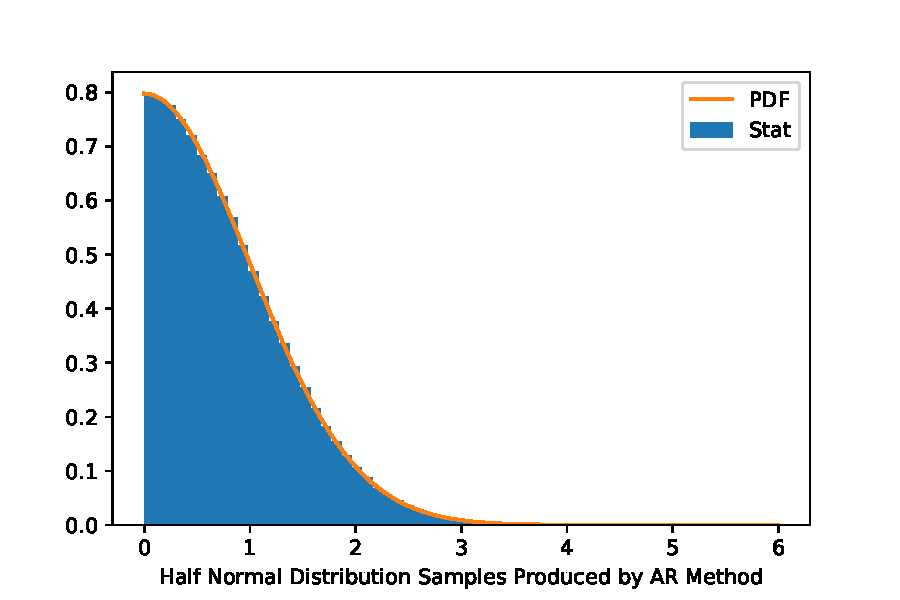
\includegraphics[width=0.45\textwidth]{images/half_normal.pdf}
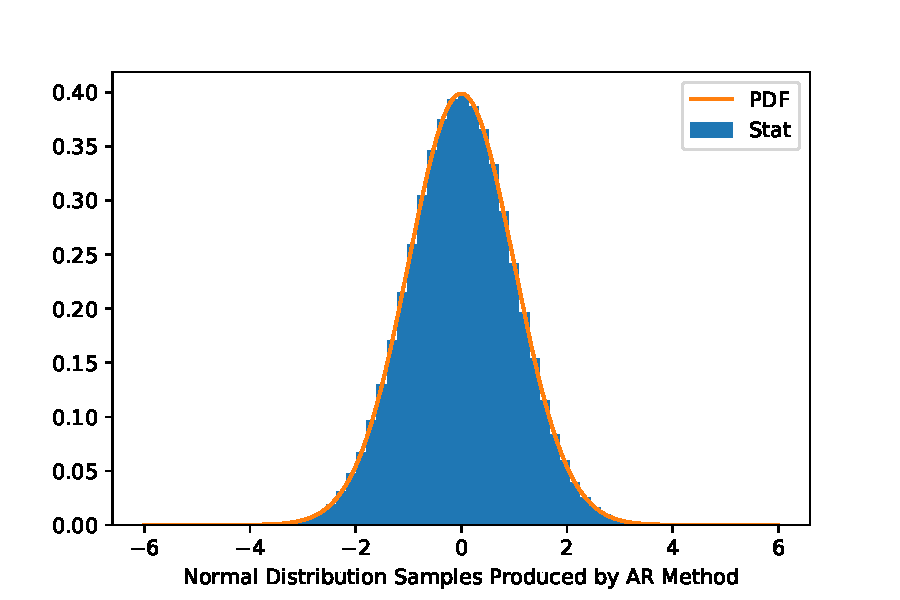
\includegraphics[width=0.45\textwidth]{images/normal.pdf}
\caption{AR法抽样生成的标准半正态分布(左,算法
    \ref{alg::sample_harl_normal})和标准正态分布(右,算法
    \ref{alg::sample_normal})的抽样统计结果和各自的PDF对比。可见抽样
  质量不错。}
\label{fig::AR_half_and_normal}
\end{figure}

我们可以如图\ref{fig::AR_region}那样绘制出用AR法抽取半正态分布的接受和
拒绝区域,它们分别是$u \leq g(-\ln x)$和$u > g(-\ln x)$,也即曲线$g(-\ln
x)$的上下部分。而常数$c$就是接受区域的面积。

注意产生目标抽样的办法肯定不止一个。我们上面严格按照AR的算法流程,先用
逆变换产生了$h$的指数分布,然后再计算$g$并通过独立的均匀分布来判定接受
或拒绝。这里产生$h$的时候用了一个log运算,产生$g$的时候做了一次指数运
算。这两个运算都是代价较高的。特别是log运算。注意到$g$本质上也是一个变
换后的指数分布,所以如果我们有一个很好的指数分布生成程序,那么可以将具
体的算法调整为各自独立地产生两个指数分布,然后对$g$产生的分布做一个变
换,再执行接受拒绝判断。具体算法见\ref{alg::sample_harl_normal_v2}。
\begin{figure}[!ht]
\centering
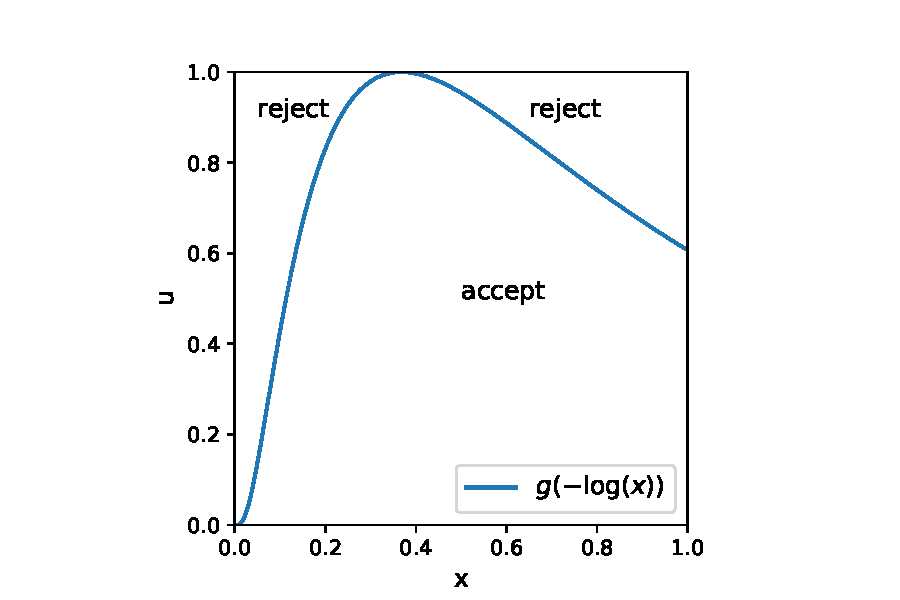
\includegraphics[width=0.7\textwidth]{images/AR_region.pdf}
\caption{AR法抽样生成的标准半正态分布的接受(accept)和拒绝(reject)区域}
\label{fig::AR_region}
\end{figure}

\begin{minipage}[!ht]{0.8\textwidth}
\vspace{3ex}
\refstepcounter{alg}
\label{alg::sample_harl_normal_v2}
\begin{center}
 算法 \arabic{chapter}.\arabic{alg} AR法抽取标准半正态分布(基于快速指
   数分布生成器)
\end{center}
\small
\begin{tabular}{lll}
  \hei 输入&N&实际抽样总数\\
  \hei 输出&k&实际接受样本总数\\
  &X&输出服从标准半正态分布的样本(前k个有效)
\end{tabular}
\begin{lstlisting}[style = python]
def sample_half_normal_v2(N):
# N, 实际采样数
    k = 0  # 实际接受总数
    X = stats.expon.rvs(size=N)  
    G = stats.expon.rvs(size=N)  # 产生两个独立的beta(1)
    for i in range(N):
        if (X[i] - 1)**2/2 <= G[i]:  # 等价于在g的条件下接受
            X[k] = X[i]   # 将采样记下来
            k = k + 1
    return k, X
\end{lstlisting}
\end{minipage}

\section{挤压算法}

我们已经注意到在抽取半正态分布时,每个样本平均需要执行
$2\sqrt{\frac{2e}{\pi}} \approx 2.631$次函数求值,一次指数运算和一次对
数运算,还得丢弃一部分。如果我们能稍微减少一些这些基本函数运算,也可以
显著降低计算代价。Marsaglia于1977年\cite{Marsaglia1977The}提出一个非常
简单但却是有效的思想,挤压算法(squeeze)。在AR法中,我们主要的计算量
来自要和$g(z)$比大小,但$g(z)$本身的计算是高代价的。如果我们能够构建关
系
\begin{equation}
  g_L(z) \leq g(z) \leq g_U(z), z \in [a, b],
\label{eq::squeeze}
\end{equation}
这里区间$[a, b]$是我们的抽样范围。而且$g_L(z)$和$g_U(z)$都是便于计算的
函数,那么对是否小于$g(z)$的判定就可以先用这两个界函数过滤一下。如果这
两个界充分接近$g(z)$,那么有很大机率,我们根本不需要再计算$g(z)$了。也
即可以将AR法的基本步骤改为:
\begin{enumerate}
\item 产生服从分布$h(z)$的随机变量$Z$;
\item 产生服从$U(0, 1)$的随机变量$U$;
\item 若$U \leq g_L(Z)$,返回$Z$;
\item 否则,若$U \leq g_U(Z)$并且$U \leq g(Z)$,返回
  $Z$,否则放弃,返回第1步。
\end{enumerate}

事实上,
\begin{equation}
  P(\mbox{计算}g(Z)) = P(g_L(Z) < U < g_U(Z)).
  \label{eq::squeeze_pg}
\end{equation}
我们用$S$表示$U \leq g(Z)$的事件,分别用$S_L$和$S_U$表示$U \leq
g_L(Z)$和$U \leq g_U(Z)$的事件,则
\begin{eqnarray}
  P(S_L) &=& \int_a^b \max\{0, g_L(z)\}h(z)dz,\\
  \label{eq::squeeze_psl}
  P(S_U) &=& \int_a^b \min\{1, g_U(z)\}h(z)dz,
  \label{eq::squeeze_psu}
\end{eqnarray}
再由\ref{eq::squeeze_pg}, 有
\begin{equation}
  P(\mbox{计算}g(Z)) = P(S_U) - P(S_L).
  \label{eq::squeeze_pg2}
\end{equation}
即在一次抽样中,要计算$g$的概率就是这么多。我们还可以令$N$为重复一次成功抽取中计算
$g(Z)$的次数,则
\begin{equation}
  E[N] = P(\bar{S}_LS_U | \bar{S})\left(\frac{1}{P(S)} - 1\right)
  + P(\bar{S}_LS_U | S).
  \label{eq::squeeze_en}
\end{equation}
这里$\bar{S}_L$和$\bar{S}$表示$U > g_L(Z)$和$U > g(Z)$,即补
事件。由条件概率公式,
\begin{equation}
  P(\bar{S}_LS_U | \bar{S}) = \frac{P(S_U) - P(S)}{1 - P(S)},
  \label{eq::squeeze_r:}
\end{equation}
和
\begin{equation}
  P(\bar{S}_LS_U | S) = \frac{P(S) - P(S_L)}{P(S)},
  \label{eq::squeeze_a}
\end{equation}
有
\begin{equation}
  E[N] = \frac{P(S_U) - P(S_L)}{P(S)}.
  \label{eq::squeeze_en_result}
\end{equation}
其中,由定义,
\begin{equation}
  P(S) = \int_a^b g(z)h(z)dz = \frac{1}{c}.
  \label{eq::squeeze_ps}
\end{equation}
用这个公式可以估计一下大概要实际抽样多少次。

经常遇到的指数和对数函数估计式如下,对指数函数,
\begin{equation}
  1 - z \leq e^{-z} \leq 1 - z + \frac{z^2}{2}, z \geq 0;
  \label{eq::squeeze_exp}
\end{equation}
对数函数
\begin{equation}
  \frac{z - 1}{z} \leq \ln z \leq -1 + z, z \geq 0.
\end{equation}

\begin{example} {\hei 对半正态抽样采用挤压法} 在算法\ref{alg::sample_harl_normal}中,我们需要计算
  $$
  g(z) = e^{-\frac{(z - 1)^2}{2}},
  $$
  现令
  \begin{equation}
    g_L(z) = 1 - \frac{(z - 1)^2}{2},
    \label{eq::squeeze_ex_gl}
  \end{equation}
  以及
  \begin{equation}
    g_U(z) = 1 - \frac{(z - 1)^2}{2} + \frac{(z - 1)^4}{8}
    = g_L(z) + \frac{(z - 1)^4}{8}.
    \label{eq::squeeze_ex_gu}
  \end{equation}
  则
  \begin{eqnarray}
    P(S_L) &=& \frac{1}{2} + (1 + \sqrt{2})e^{-(1 + \sqrt{2})} \approx 0.7159,\\
    P(S_U) &=& \frac{13}{8} - 16e^{-3} \approx 0.8284,
  \end{eqnarray}
  以及
  \begin{equation}
    P(\mbox{计算}g(Z) = P(S_U) - P(S_L) \approx 0.1125,
  \end{equation}
  同时平均每生成一个成功采样需要计算$g(z)$的次数为
  \begin{equation}
    E[N] = \frac{P(S_U) - P(S_L)}{P(S)}
    = (P(S_U) - P(S_L)) \times c \approx 0.1480.
  \end{equation}
  于是每成功生成一个采样需要计算$g(Z)$的次数从$c \approx 1.3155$下降到
  了$0.1480$,效果还是很显著的。从图\ref{fig::squeeze_half_normal}也可
  以看到需要计算$g(Z)$的范围大大减少。
  \label{example::squeeze_half_normal}
\end{example}

\begin{figure}[!ht]
\centering
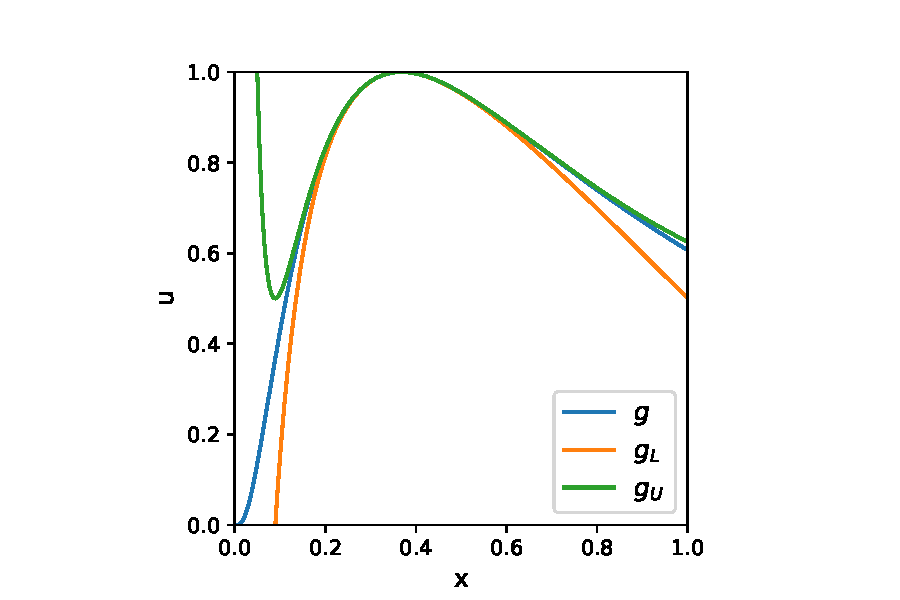
\includegraphics[width=0.7\textwidth]{images/squeeze.pdf}
\caption{用AR法抽取半正态分布,挤压后在$g_L$和$g_U$之间的区域才实际需要计算$g(Z)$。}
\label{fig::squeeze_half_normal}
\end{figure}

可以想象,高效率随机抽样这个问题既是计算机模拟的核心底层操作,又是一个
没有止境的操作。同时,和随机数生成一样,它还涉及到很多具体的理论和技术
细节。可以预见,随着计算机模拟的重要性不断提升,这些基础核心问题也会日
益受到重视。我们到这里只介绍了最基本的算法思想,更多的内容,请参阅
\cite{Fishman1995Monte}的第2 \~ 4章。同时要注意这方面不断有新文献产生。

\section{正态分布抽取}
在本章最后,我们单独介绍一个特别重要的分布的抽样方法——正态分布。服从
$N(\mu, \sigma^2)$的正态分布相应的PDF为
\begin{equation}
  f(z) = \frac{1}{\sqrt{2\pi \sigma^2}} e^{\frac{-(z -
      \mu)^2}{2\sigma^2}}, \sigma^2 > 0, z \in \mathbb{R}.
\end{equation}
关于正态分布的一些性质,大家应该是熟知的:
\begin{enumerate}
\item 若$U$服从正态分布$N(0, 1)$,
  则$Z = \mu + \sigma U$服从$N(\mu, \sigma^2)$分布;
\item 若$Z_1, Z_2, \cdots, Z_n$是分别服从$N(\mu_1, \sigma_1^2),
  N(\mu_2, \sigma_2^2), \cdots, N(\mu_n, \sigma_n^2)$的独立随机变量,
  则$Z = Z_1 + Z_2 + \cdots + Z_n$服从分布$N(\mu_1 + \mu_2 +
  \cdots + \mu_n, \sigma_1^2 + \sigma_2^2 + \cdots + \sigma_n^2)$.
\end{enumerate}
根据以上的性质,我们知道我们只需要抽样生成$N(0, 1)$就足够了。我们之前
已经介绍了如何由AR法产生半正态分布,进而抽样改造成标准正态分布。下面我
们再介绍两种简单的抽取方法。假设
\begin{equation}
  Z_n = \sqrt{12/n}(X_1 + X_2 + \cdots + X_n),
  \label{eq::normal_naive}
\end{equation}
其中$X_i$是独立的服从$U(-\frac{1}{2}, \frac{1}{2})$的随机变量,那么显然有
对$i = 1, 2, \cdots, n$, $E[X_i] = 0$, 且
$$
D[X_i] = \int_{-\frac{1}{2}}^{\frac{1}{2}}x^2 dx = \frac{1}{12}.
$$
也即$Z_n$的头两阶矩和$N(0, 1)$一致。当$n \to \infty$时,$Z_n \sim N(0,
1)$. 如果我们取$n = 12$,那么甚至连根号都不用计算了,但是这时我们发现
$Z_{12}$实际上分布在$(-6, 6)$区间而不是$\mathbb{R}$. 这个方法只有在
条件简陋的情况下可以用一下。

第二个方法可以总结成一个定理,由Box and Muller在1958年\cite{Box1958A}提出:
\begin{theorem}{}
  令随机变量$U$和$V$分别服从$U(0, 1)$和$E(1)$(表示参数为1的指数分布),那么
  \begin{equation}
    X = \sqrt{2 V}\cos 2\pi U
    \label{eq::normal_box_muller_xi}
  \end{equation}
  和
  \begin{equation}
    Y = \sqrt{2 V}\sin 2\pi U
    \label{eq::normal_box_muller_eta}
  \end{equation}
  是服从$N(0, 1)$的独立随机变量。

  \noindent{\hei 证明:} 注意到
  $$
  f_U = 1, f_V = e^{-v}.
  $$
  再令
  $$
  x = \sqrt{2v}\cos 2\pi u, y = \sqrt{2v}\sin 2\pi u,
  $$
  则有  
  $$
  2 v = x^2 + y^2
  $$
  和
  $$
  \tan 2 \pi u =\frac{y}{x}.
  $$
  因此$X$和$Y$的联合分布函数为
  \begin{equation}
    f_{X, Y}(x, y) = f_{U, V}(u(x, y), v(x,
    y))\left|\frac{\partial u}{\partial x}\frac{\partial v}{\partial
      y} - \frac{\partial u}{\partial y}\frac{\partial v}{\partial
      x}\right| = \frac{1}{2 \pi}e^{-\frac{x^2 + y^2}{2}}.
  \end{equation}
  则$f_X$和$f_Y$各自的边界分为标准正态分布。证毕。
  \label{thm::normal_box_muller}
\end{theorem}

而当前已知生成正态分布最快的方法是由Marsaglia在1964年
\cite{Marsaglia1964A}提出的rectangle-wedge-tail方法,并在1972年由
Ahrens和Dieter修改成RT算法\cite{Dieter1973A}。但是他们的方法都需要准备
大量的预制表格,这一系方法实现比较繁琐。在不用查表的情况下,生成正态分
布最快的方法,它是由Ahrens和Dieter在1988年提出的NA算法
\cite{Ahrens1988Efficient}。有兴趣的同学可自行参阅相应文献。


\chapter{Monte Carlo法:估算体积和计数}

这一章我们开始介绍Monte Carlo法的基础理论。从如何估算一个多维欧氏空间
中的有界区域的体积(Volumn)开始。更一般的问题则是在相同区域中估算积分。
当区域或目标函数复杂时,Monte Carlo法具有经典数值方法所无法取代的优势。
而计数估计(Evaluating count)则是另一个非常重要的问题。它的一个来源是
当我们有时需要估计一个元素数量为$m$的集合中具有指定性质的子集的个数。
但这种估算的经典算法往往是关于$m$指数增长的。也即我们无法精确地列举全
部子集,然后进行计数。Monte Carlo法在这种情形下,也具有优势。

尽管体积估算和计数估计一个是连续,一个是离散。但实际上这是一类基础问题
的不同方面。它们实际上的理论和技巧是相通的。甚至我们有时直接将计数包含
进体积的概念之中以简化叙述。

\section{体积估计}

令$\mathscr{R}$是一个包含在$m$维超立方体
\begin{equation}
  \mathscr{J}^m = [0, 1]^m = [0, 1] \times \cdots \times [0, 1]
  \label{eq::hyper_cube}
\end{equation}
中的$m$维有界区域,且其体积$\lambda(\mathscr{R})$未知。而对于一般的有
界区域,我们假设可以通过适当的变换将其映射进$\mathscr{J}^m$。如果我们
能够产生$m$维点列
\begin{equation}
  \mathscr{K}_{m, n} = \left\{\vec{x}^{(j)} = (x_1^{(j)}, x_2^{(j)},
  \cdots, x_m^{(j)}) \in \mathscr{J}^m, j = 1, \cdots, n\right\},
  \label{eq::m_d_random_number}
\end{equation}
则$\lambda(\mathscr{R})$可以用$\bar{\lambda}_n(\mathscr{R})$来逼近。伪
代码如算法\ref{alg::volumn}。

\begin{minipage}[!ht]{0.8\textwidth}
\vspace{3ex}
\refstepcounter{alg}
\label{alg::volumn}
\begin{center}
 算法 \arabic{chapter}.\arabic{alg} 估算体积
\end{center}
\small
\begin{tabular}{ll}
  \hei 目标&估算$\lambda(\mathscr{R})$.\\
  \hei 输入&包含在$\mathscr{J}^m$中的区域$\mathscr{R}$, 以及$n$个计值点.\\
  \hei 输出&$\bar{\lambda}_n(\mathscr{R})$.
\end{tabular}
\begin{enumerate}
\item $j = 1$, $S = 0$.
\item While $j \leq n$:
  \begin{enumerate}
    \item 从$\mathscr{K}_{m, n}$中产生$\vec{x}^{(j)}$.
    \item $\phi(\vec{x}^{(j)}) = 0$.
    \item If $\vec{x}^{(j)} \in \mathscr{R}, \phi(\vec{x}^{(j)}) = 1$.
    \item $S = S + \phi(\vec{x}^{(j)})$.
    \item j = j + 1.
  \end{enumerate}
  \item 计算$\bar{\lambda}_n(\mathscr{R}) = S/n$.
\end{enumerate}
\end{minipage}

这里具体的$\bar{\lambda}(\mathscr{R})$的数值精度依赖$\mathscr{R}$和
$\mathscr{K}_{m, n}$的性质。比如如果取均匀划分的网格点,则有
\begin{equation}
  \mathscr{K}_{m, n} = \left\{\vec{x} = (x_1, \cdots, x_m) : x_i =
  \frac{z_i + \frac{1}{2}}{k}, z_i = 0, \cdots, k - 1, i = 1, \cdots,
  m, n = k^m\right\}.
  \label{eq::m_d_lattice}
\end{equation}
这个公式的含义是格点在第$i$维的坐标$x_i$可以取$z_i = 0, \cdots, k - 1$
中的任何一个,可以重复取,这样的组合一共有$n = k^m$个,每一组都代表了
一个$m$维超单位正方体$\mathscr{J}^m$中的均匀格点。比如我们不难画出2维
的特例(见图\ref{fig::2_d_lattice})。可以看到$k$代表了在一个维度上的均匀格点个数。每一个格点,均是
一个体积为$1 / k^m = 1 / n$的小超正方体的中心。因此落在
$\mathscr{R}$内的格点个数$S$可以估算出$\mathscr{R}$的体积
$$
\lambda(\mathscr{R}) \approx \bar{\lambda}_n(\mathscr{R}) =
\frac{S}{n}.
$$

\begin{figure}[!ht]
\centering
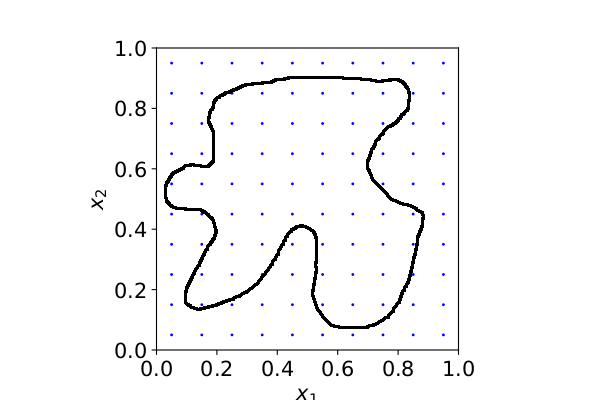
\includegraphics[width=0.7\textwidth]{images/lattice.png}
\caption{二维单位正方体内的均匀网格,$k = 10$。中间不规则区域表示$\mathscr{R}$。}
\label{fig::2_d_lattice}
\end{figure}

如果我们用$s(\mathscr{R})$表示二维区域$\mathscr{R}$的边长,那么通过观
察不难看出绝对误差有上界估计
\begin{equation}
  \left|\bar{\lambda}_n(\mathscr{R}) - \lambda(\mathscr{R})\right|
  \leq \frac{s(\mathscr{R})}{k}.
  \label{eq::2_d_absolute_error}
\end{equation}
事实上,包含了不确定的绝对误差部分最大不会超过长度为$s(\mathscr{R})$,
宽度为$1/k$的条状地带面积。而更一般的,如果用$s(\mathscr{R})$表示一个
$m$维区域$\mathscr{R}$的表面积,则对应的绝对误差界也是
(\ref{eq::2_d_absolute_error})。由$n = k^m$,有
\begin{equation}
  \left|\bar{\lambda}_n(\mathscr{R}) - \lambda(\mathscr{R})\right|
  \leq \frac{s(\mathscr{R})}{n^{\frac{1}{m}}},
  \label{eq::m_d_absolute_error}
\end{equation}
也即误差收敛率随$m$上升而下降。或者说,如果要保证误差小于$\varepsilon \in (0, 1)$,则
需要
$$
n(\varepsilon) =
\left\lceil\left(\frac{s(\mathscr{R})}{\varepsilon}\right)^m\right\rceil
$$
个点才能保证。

而Monte Carlo方法只改变其中一步,即将序列$\{\vec{x}^{(1)}, \cdots,
\vec{x}^{(n)}\}$从一个确定的序列,改成一系列在$\mathscr{J}^m$中均匀分
布的独立随机变量
$$
\vec{X}^{(j)} = \{X_1^{(j)}, \cdots, X_m^{(j)}\}, j = 1, \cdots, n.
$$也即,$X_i$的PDF均为$U(0, 1)$. 做相应修改后的算法\ref{alg::volumn}就
是Monte Carlo算法,简称MC,或者,也称作标准Monte Carlo采样(standard
Monte Carlo sampling)。我们用算法\ref{alg::MC}表示。

\begin{minipage}[!ht]{0.8\textwidth}
\vspace{3ex}
\refstepcounter{alg}
\label{alg::MC}
\begin{center}
 算法 \arabic{chapter}.\arabic{alg} MC
\end{center}
\small
\begin{tabular}{ll}
  \hei 目标&估算$\lambda(\mathscr{R})$.\\ \hei 输入&包含在
  $\mathscr{J}^m$中的区域$\mathscr{R}$, 样本尺寸$n$, 置信水平$1 -
  \delta$. \\
  \hei 输出&估计值$\bar{\lambda}_n(\mathscr{R})$, 方差$\mathrm{var} \bar{\lambda}_n(\mathscr{R})$ 以及置信区间.
\end{tabular}
\begin{enumerate}
\item $j = 1$, $S = 0$.
\item While $j \leq n$:
  \begin{enumerate}
    \item 生成$\vec{X}^{(j)}$.
    \item $\phi(\vec{X}^{(j)}) = 0$.
    \item If $\vec{X}^{(j)} \in \mathscr{R}, \phi(\vec{X}^{(j)}) = 1$.
    \item $S = S + \phi(\vec{X}^{(j)})$.
    \item j = j + 1.
  \end{enumerate}
\item 做统计分析:
  \begin{enumerate}
  \item 计算$\bar{\lambda}_n(\mathscr{R}) = S/n$作为$\lambda(\mathscr{R})$的点估计.
  \item 计算$V[\bar{\lambda}_n(\mathscr{R})] = (S / n)(1 - S / n) / (n - 1)$ 作为$\mathrm{var~} \bar{\lambda}_n(\mathscr{R})$的点估计.
  \item 根据置信水平计算百分之$100 \times (1 - \delta)$的置信区间.
  \end{enumerate}
\end{enumerate}
\end{minipage}

注意到$\vec{X}^{(1)}, \cdots \vec{X}^{(n)}$均为独立随机变量且PDF为
\begin{equation}
  f(\vec{x}) = \left\{
  \begin{array}{ll}
    1, & 0 \leq x_i \leq 1, i = 1, \cdots, m,\\
    0, & \mbox{其他}.
  \end{array}
  \right.
  \label{eq::MC_X_PDF}
\end{equation}
因此$\phi(\vec{X}^{(1)}), \cdots, \phi(\vec{X}^{(n)})$为独立的
Bernoulli分布随机变量,满足
\begin{equation}
  P\{\phi(\vec{X}^{(j)}) = 1\} = \int_{\mathscr{R}} f(\vec{x}) dx =
  \lambda(\mathscr{R})
  \label{eq::MC_phi_X}
\end{equation}
且
\begin{equation}
  P\{\phi(\vec{X}^{(j)}) = 0\} = \int_{\mathscr{J}^m \backslash
    \mathscr{R}} f(\vec{x}) dx = 1 - \lambda(\mathscr{R}), j = 1, \cdots, n.
  \label{eq::MC_phi_X_R}
\end{equation}
所以,$S = \phi(\vec{X}^{(1)}) + \cdots + \phi(\vec{X}^{(n)})$服从二项分布
\begin{equation}
  P\{S = i\} = f_i(n, \lambda) = \binom{n}{i} \lambda^i (1 -
  \lambda)^{n - i}, \lambda = \lambda(\mathscr{R}), i = 0, \cdots, n.
  \label{eq::MC_Bernoulli}
\end{equation}
二项分布的期望和方差分别是$E[S] = n \lambda$和$\mathrm{var~} S =
n\lambda(1 - \lambda)$. 于是$\bar{\lambda}_n =
\bar{\lambda}_n(\mathscr{R})$可以看作是$\lambda$的一个无偏估计,且有
\begin{equation}
  \mathrm{var~} \bar{\lambda}_n = \frac{1}{n^2} \mathrm{var~} S =
  \lambda (1 - \lambda) / n.
  \label{eq::var_lambda_bar}
\end{equation}
注意其实$\lambda$是未知量,因此我们并不能用公式(\ref{eq::var_lambda_bar})来估算误差。

\section{误差和样本大小}

首先我们要明确,对Monte Carlo法而言,收敛指的是依概率$1$收敛,也即
\begin{equation}
  P\left\{\lim_{n \to \infty} \bar{\lambda}_n = \lambda \right\} = 1.
\end{equation}
因此,所谓误差也是点估计或区间估计意义上的。比如算法\ref{alg::MC}中的
$V[\bar{\lambda}_n(\mathscr{R})]$就是$\mathrm{var~} \bar{\lambda}_n$的
一个无偏估计,因为
\begin{equation}
  \begin{array}{rcl}
  E[(S / n) (1 - S / n)] &=&  \displaystyle \frac{1}{n} E[S] -
  \frac{1}{n^2}(\mathrm{var~} S + E^2[S])\\\\
  &=& \displaystyle\frac{\lambda (1 - \lambda) (n - 1)}{n}.
 \end{array}
\end{equation}

而$\sqrt{V[\bar{\lambda}_n]}$被称为$\bar{\lambda}_n$的标准误差(standard
  error)。有时被用作$\bar{\lambda}_n$的统计误差的一个粗略估计,不过由
于$V[\bar{\lambda}_n]$本身就是一个估计量,因此要慎重使用。要系统考虑误
差的分布,则需要统计学理论,我们陆续会选择一些重要的(或者对我们而言有
  用的)介绍。

\begin{theorem}{\hei \bf Chebshev不等式}
  令$Z$是一个累积分布为$F(z)$的随机变量,$z \in (-\infty, \infty)$。且$E[Z] = 0$,
  $\sigma^2 = \mathrm{var~} Z = E[Z^2] < \infty$。则对$\beta > 0$,有
  \begin{equation}
    P\left\{\frac{|Z|}{\sigma} \geq \beta\right\} \leq \frac{1}{\beta^2}.
    \label{eq::cheb_ineq}
  \end{equation}
  \label{thm::cheb_ineq}
\end{theorem}

\begin{proof} 对$\varepsilon > 0$,有
  \begin{equation}
    \begin{array}{rcl}
    P\{|Z| \geq \varepsilon\} &=& \displaystyle
    \int_{-\infty}^{-\varepsilon}d F(z) + \int_{\varepsilon}^{\infty}d
    F(z) \\\\ &\leq& \displaystyle
    \int_{-\infty}^{-\varepsilon}\frac{z^2}{\varepsilon^2} d F(z)
    + \int_{\varepsilon}^{\infty}\frac{z^2}{\varepsilon^2} d F(z)\\\\
    &\leq& \displaystyle \frac{1}{\varepsilon^2}\int_{-\infty}^{\infty}z^2 d F(z)
    = \frac{\sigma^2}{\varepsilon^2}.
    \end{array}
  \end{equation}
  取$\beta = \varepsilon / \sigma$即得(\ref{eq::cheb_ineq})。
\end{proof}

现取$Z = S / n - \lambda$和$\sigma^2 = \lambda(1 - \lambda) / n$,得
\begin{equation}
  P\{|\bar{\lambda}_n - \lambda| < \varepsilon\} \geq 1 - \lambda(1 - \lambda) / n \varepsilon^2.
  \label{eq::col_cheb_ineq}
\end{equation}
即
\begin{equation}
  \lim_{n \to \infty} P\{|\bar{\lambda}_n - \lambda| \geq \varepsilon\} = 0.
  \label{eq::cov_pro}
\end{equation}
上式称为概率收敛(convergence in probability),由依概率1收敛可以导出
概率收敛,但反过来不行。它比依概率1收敛(convergernce with 
  probability 1,缩写w.p.1)要弱。但这里实际给出了一个收敛性和样本大小$n$之
间的关系。不过这里再大的$n$都不能\CJKunderdot{确保}误差小于
$\varepsilon$。为了正确的体现和评估随机性,我们需要引入置信水平
(confidence level)$1 - \delta$,$0 < \delta < 1$,由Chebyshev不等式,
当
\begin{equation}
  n \geq n_C(\varepsilon, \delta, \lambda) = \lceil \lambda (1 -
  \lambda) / \delta \varepsilon^2 \rceil
  \label{eq::cheb_ineq_est}
\end{equation}
时,误差满足
\begin{equation}
  P\{|\bar{\lambda}_n - \lambda| < \varepsilon\} \geq 1 - \delta.
  \label{eq::abs_error_crit}
\end{equation}
我们称其为绝对误差准则(absolute error criterion)。注意到$\lambda(1 -
\lambda) \leq 1 / 4$,故有最坏情形样本数(the worst-case sample size)
\begin{equation}
  n_C(\varepsilon, \delta) = \lceil \frac{1}{4 \delta \varepsilon^2}\rceil,
  \label{eq::wc_sample_s}
\end{equation}
对所有$\lambda \in [0, 1]$。

公式(\ref{eq::wc_sample_s}) 表达了Monte Carlo法最重要的性质,
$n_C(\varepsilon, \delta, \lambda)$和维数$m$无关。而在实际计算中,由于
随机投点本身是一个$O(m)$的操作,且在每个维度上我们要通过计算来判断
$\vec{X}$是否属于$\mathscr{R}$,这些操作加起来不超过$O(m^\beta)$,
$\beta \geq 1$。故实际在程序中估算绝对误差界的代价是
$$
O([m^\beta \frac{\lambda (1 - \lambda)}{\delta \varepsilon^2}])
= O(\frac{m^\beta}{4 \delta \varepsilon^2}).
$$
仍然是一个关于$m$的多项式时间算法,而相应精确逼近算法关于$m$是指数时间的。

尽管公式(\ref{eq::wc_sample_s})给出了一个样本数的估计,但这个估计明
显是过宽的。实际上的样本数需求要远小于这个估计。为此我们考虑根据中心极
限定理,当$n \to \infty$时,特征量
$$
\frac{S - n \lambda}{[n \lambda (1 -
  \lambda)]^{\frac{1}{2}}}
$$
是服从标准正态分布
\begin{equation}
  \Phi(z) = (2 \pi)^{-\frac{1}{2}}\int_{-\infty}^z e^{-\frac{y^2}{2}} dy, -\infty < z < \infty,
  \label{eq::cdf_std_normal}
\end{equation}
也即$N(0, 1)$分布。令
\begin{equation}
  n_N(\varepsilon, \delta, \lambda) = \left\lceil \lambda (1 -
  \lambda) \left[\frac{\Phi^{-1}(1 -
      \frac{\delta}{2})}{\varepsilon}\right]^2\right\rceil,
  \label{eq::es_sample_s}
\end{equation}
其中
\begin{equation}
  \Phi^{-1}(\theta) = \inf\left[z : (2 \pi)^{-\frac{1}{2}}
    \int_{-\infty}^z e^{-\frac{y^2}{2}} dy = \theta, 0 < \theta < 1\right].
\end{equation}
于是当$\varepsilon \to 0$, 公式(\ref{eq::es_sample_s})给出了在参数
$(\varepsilon, \delta)$下,绝对误差满足
\begin{equation}
  \lim_{\varepsilon \to 0} P\left\{\frac{\left|\frac{S}{n_N(\varepsilon,
      \delta, \lambda)} - \lambda\right|}{\varepsilon} \leq 1\right\} = 1 - \delta
  \label{eq::es_pro_abs_error}
\end{equation}
的样本数。而对应的最坏情形样本数是
\begin{equation}
  n_N(\varepsilon, \delta) = \left\lceil \left[\frac{\Phi^{-1}(1 -
      \frac{\delta}{2})}{2\varepsilon}\right]^2\right\rceil.
  \label{eq::es_worst_sample_s}
\end{equation}

我们可以比较在$\delta = 0.001$, $0.01$和$0.05$下,
$$
\frac{n_C}{n_N} = \frac{1}{\delta\left[\Phi^{-1}(1 - \frac{\delta}{2})\right]^2}
$$的值分别是$92.36$, $15.07$和$5.21$。可见这个比例还是很大的。不过这么
估计也有比较严重的问题。因为我们实际上就把$S / n$当作正态分布计算了,
而这个只是一个概率极限情形。因此,当$n$不够大(注意这里逻辑上有矛盾),
或者$\varepsilon$太小时,这个结果都有很大的误差。一个弥补的办法是故意
高估$n$,比如有人建议总是取两倍的$n_N$。而更加靠谱的估计,来自
Hoeffding于1963年的工作\cite{Wassily1963Probability}。(以下部分只要了
  解结论,不作要求。)

\begin{theorem}{\bf Hoeffding 1963}
  令$Z_1, \cdots, Z_n$是独立随机变量且
  $$
  \mu_i = E[Z_i] \in (0, 1), P\{0 \leq Z_i \leq 1\} = 1, i = 1, \cdots, n.
  $$
  令$\mu = (\mu_1 + \cdots + \mu_n) / n$。 则对$0 < \varepsilon < 1 -\mu$,和
  $\bar{Z}_n = (Z_1 + \cdots + Z_n) / n$,
  \begin{eqnarray}
    P\{\bar{Z}_n - \mu \geq \varepsilon\} &\leq& e^{n w(\varepsilon, \mu)} \\
    \label{eq::hoeffding1963_1}
    & \leq & e^{-\mu g(\mu) \varepsilon^2} \\
    \label{eq::hoeffding1963_2}
    & \leq & e^{-2 n \varepsilon^2},
    \label{eq::hoeffding1963_3}
  \end{eqnarray}
  其中
  \begin{equation}
    w(\varepsilon, \mu) = (\mu + \varepsilon) \log
    \left(\frac{\mu}{\mu + \varepsilon}\right) + (1 - \mu -
    \varepsilon) \log\left(\frac{1 - \mu}{1 - \mu - \varepsilon}\right),
    \label{eq::hoeffding1963_w}
  \end{equation}
  以及
  \begin{equation}
    g(\mu) =
    \left\{
        \begin{array}{ll}
          \displaystyle \frac{1}{1 - 2 \mu} \log\left(\frac{1 -
            \mu}{\mu}\right),& \mbox{若} 0 < \mu <
          \frac{1}{2}\\\\ \displaystyle \frac{1}{2\mu(1 - \mu)},&
          \mbox{若} \frac{1}{2} \leq \mu < 1.
        \end{array}\right.
        \label{eq::hoeffding1963_g}
  \end{equation}
  \label{thm::Hoeffding1963}
\end{theorem}

\begin{corollary}
  对公式(\ref{eq::hoeffding1963_w})中定义的$w(\varepsilon, \mu)$,
  \begin{equation}
    \lim_{\varepsilon \to 0} \varepsilon^{-2} w(\varepsilon, \mu) =
    -\frac{1}{2\mu(1 - \mu)}。
  \end{equation}
  \label{cor::hoeff_1}
\end{corollary}

\begin{corollary}
  函数$w(\varepsilon, y)$,$0 < \varepsilon < 1 - y$,$0 < y < 1$关于
  $y$是凹的。故有最大值$y^* \in [\max(0, \frac{1}{2} - \varepsilon),
    \frac{1}{2}]$。
  \label{cor::hoeff_2}
\end{corollary}

\begin{corollary}
  函数$w((y + v)\varepsilon, y)$,$0 < \varepsilon \leq \frac{1 - y}{y
    + v}$,$0 < y < 1$,$v \geq 0$;和函数$w((y + v)\varepsilon, 1 -
  y)$,$0 < \varepsilon \leq \frac{y}{y + v}$,$0 < y < 1$,$v > 0$,
  关于$y$都是凹的。
  \label{cor::hoeff_3}
\end{corollary}

\begin{corollary}
  对公式(\ref{eq::hoeffding1963_w})中定义的$w(\varepsilon, y)$,有
  $w(\varepsilon, y) \geq w(\varepsilon, 1 - y)$,$\varepsilon \leq y
  \leq \frac{1}{2}$。
  \label{cor::hoeff_4}
\end{corollary}

以上证明略。自行参考\cite{Fishman1995Monte}第24页、附录及Hoeffding原文。
该定理可导出一系列有用的结论。比如样本量的估计:
\begin{equation}
  n_H(\varepsilon, \delta) =
  \left\lceil\frac{2\log(\frac{2}{\delta})}{4\varepsilon^2}\right\rceil.
  \label{eq::hoeff_sample_no_1}
\end{equation}
以及对$\varepsilon < \min\{\mu, 1 - \mu\}$(这里$\mu = \lambda$),有
\begin{equation}
  n_H(\varepsilon, \delta) =
  \left\lceil\frac{\log(\frac{\delta}{2})}
                   {\sup_{\varepsilon \leq v \leq 1 - \varepsilon} w(\varepsilon, v)}
                   \right\rceil.
  \label{eq::hoeff_sample_no_2}
\end{equation}
这里公式(\ref{eq::hoeff_sample_no_2})分母中的最大值可以用数值方法求
解。这两个估计一般认为是比$n_N$更精确的估计。

\section{置信区间}

之前我们给出了面积的一个点估计$\bar{\lambda}_n$,以及讨论在置信度
$\delta$下的一个关于偏差$\varepsilon$的样本数量估计。似乎所有关于计算
模拟的信息已经具备了,为何还要继续讨论区间估计呢?或者说区间估计难道不
就是
$$
P\{|\bar{\lambda}_n - \lambda| \leq \varepsilon\} = 1 - \delta
$$
吗?这个结果有两个比较可疑的地方,一个是这个区间居然是对称的;另一个是
这个估计居然和$\lambda$无关。
%% 我们倒是学过另一个点估计值
%% $V[\bar{\lambda}_n]$,并称它的算术平方根为标准误差,作为一个误差的估计。
%% 我们注意到它也是对称的,但它和$S$,进而和$\lambda$有关。通过我们的作业,
%% 我们了解到$\sqrt{V[\bar{\lambda}_n]}$和$\bar{\lambda}_n$具有相关性,也就
%% 是$\bar{\lambda}_n$越接近$0$,$\sqrt{V[\bar{\lambda}_n]}$会越小;
%% $\bar{\lambda}_n$越接近$1$,$\sqrt{V[\bar{\lambda}_n]}$会越大。而且这种趋
%% 势,无法通过增加$n$消除。这一点我们可以通过概率论的推导证明。
但是我们考虑一下如果一个实际的$\lambda$比较接近$0$,那么在随机投点时,
落入$\mathscr{R}$内的点数本身就相对有限,因此其频率$\bar{\lambda}_n$往
负方向\CJKunderdot{可能的}偏差就很有限。比如$\lambda = 0.005$,那么负
方向的偏差不可能大于$0.005$。但正方向的偏差却仍然服从方差分布的规律,
可以大于$0.005$。于是我们应该能观察到频率$\bar{\lambda}_n$的分布往正方
向偏的现象。图(\ref{fig::bias_lambda_n})给出了$n = 1000$时,对一个面
积为$0.005$的圆进行Monte Carlo求面积时的频率分布的统计,总共做了
$50000$组实验。我们可以看到,实际的频率分布确实是往正方向偏移的。因为
负方向根本没有偏移的空间了。

\begin{figure}[!ht]
\centering
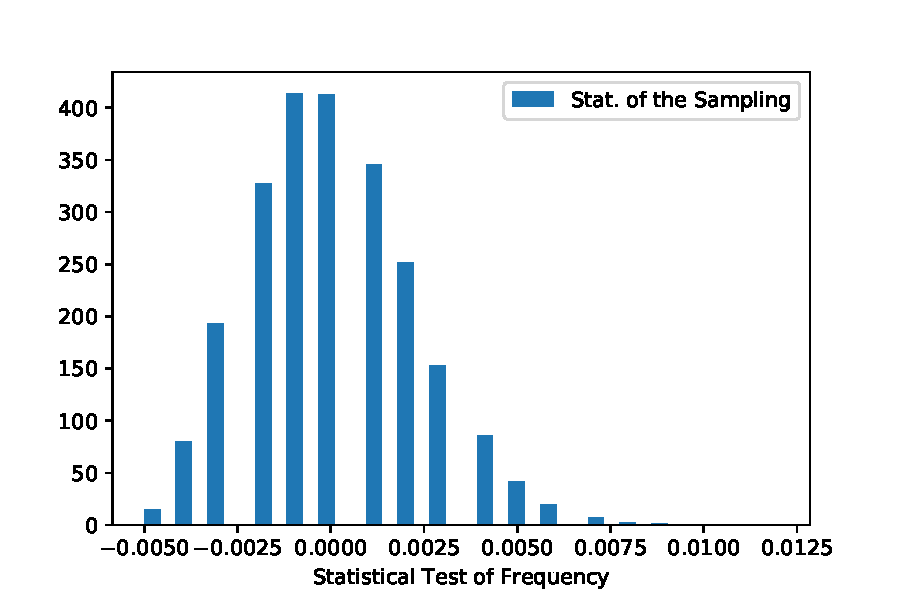
\includegraphics[width=0.7\textwidth]{images/bais_lambda_n.pdf}
\caption{对一个面积为$0.005$的圆进行Monte Carlo求面积时频率分布的统计,
  $n = 1000$,总共做了$50000$组实验。}
\label{fig::bias_lambda_n}
\end{figure}

以上这些观察提示我们,实际频率的分布和频率本身有关,同时也应该有一定的
偏移。这就是区间估计的出发点。我们希望将频数$S$也纳入统计估计,给出一
个置信区间的上下界范围。也即寻找$I_1 = I_1(S, n, \delta)$和$I_2 =
I_2(S, n, \delta)$,使得
$$
P\{I_1, I_2, \delta\} = P\{I_1 < \lambda < I_2\} \geq 1 -\delta.
$$
这里$P\{I_1, I_2, \delta\}$称为范围概率(coverage probability)或者可
靠系数(confidence coefficent)。而区间$[I_1, I_2]$称为置信区间
(confidence interval)。置信区间是比给出一个单点估计$\bar{\lambda}_n$
更加可靠的统计估计。关于二项分布的区间估计的理论和方法很多。我们这里给
出三种主要方法。

记二项分布的累计分布函数为
\begin{equation}
  F_i(n, \mu) = \sum_{j = 0}^i \binom{n}{j} \mu^j (1 - \mu)^{n - j}, 0
  < \mu < 1, i = 0, 1, \cdots, n.
  \label{eq::binomial_CDF}
\end{equation}
因此对$0 < \alpha_1 < \alpha_2 <1$,存在唯一的$\theta_1(s, n, \alpha_1)$和
$\theta_2(s, n, \alpha_2)$分别满足
\begin{equation}
  1 - F_{s - 1}(n, \theta) = \alpha_1
  \label{eq::binomial_theta_1}
\end{equation}
和
\begin{equation}
  F_s(n, \theta) = 1 - \alpha_2.
  \label{eq::binomial_theta_2}
\end{equation}
特别地,对$s = 1$,我们分别令$\theta_1 = 0$和$\theta_2 = 1$。注意到
$F_s(n, \theta)$关于$\theta$递减和关于$s$递增,所以有
$$
0 \leq \theta_1(s, n, \alpha_1) < \theta_2(s, n, \alpha_2) \leq 1.
$$
因此,若对$n$次独立的Bernolli试验,恰好成功$S$次的概率是$\mu$,则对满足
$$
1 + \alpha_1 - \alpha_2 = \delta
$$
的$\alpha_1$和$\alpha_2$,区间$[\theta_1(S, n, \alpha_1),
  \theta_2(S, n, \alpha_2)]$就是$\mu$关于置信水平$1-\delta$的范围区间,也即
$$
P\{\theta_1(S, n, \alpha_1) < \mu < \theta_2(S, n, \alpha_2)\} \geq 1 - \delta.
$$
满足上面条件的$\alpha_1$和$\alpha_2$很多,我们这里采用的是$\alpha_1
= \frac{\delta}{2}$和$\alpha_2 = 1 - \frac{\delta}{2}$. 也即我们最终取
$$
I_1(S, n, \delta) = \theta_1(S, n, \frac{\delta}{2}),
I_2(S, n, \delta) = \theta_2(S, n, 1 - \frac{\delta}{2}).
$$

为了计算$\theta_1$和$\theta_2$,我们引入不完全Beta函数\cite{Abramowitz1970Handbook}:
\begin{equation}
  1 - F_{j - 1}(n, \theta) = H_\theta(j, n - j + 1) = \frac{1}{B(j, n
    - j + 1)}\int_0^\theta z^{j - 1}(1 - z)^{n - j} dz, 0 \leq \theta \leq 1.
  \label{eq::incomplete_beta}
\end{equation}
其中$B(\cdot, \cdot)$表示Beta函数。而$H_\theta(j, n - j + 1)$实际上就
是参数为$j$和$n - j + 1$的Beta分布的累积分布函数。而所求
$$
\theta_1(S, n, \frac{\delta}{2}), \theta_2(S, n, 1 - \frac{\delta}{2})
$$
就分别是方程
$$
H_\theta(S, n - S + 1) = \frac{\delta}{2},
H_\theta(S + 1, n - S) = 1 - \frac{\delta}{2}
$$
的根。

在具体求根的时候,注意到$H_\theta$关于$\theta$的单调性,我们可以用二分
法来求解。初始含根区间可以选为$\theta_a = 0$,$\theta_b = 1$。如果要加
速收敛,可以在误差达到一定精度后采用Newton迭代。这些方法是经典数值方法,
这里不再详述,具体例子可参见讲义第四章附带代码。表
\ref{table::confidence_intervals}给了一些实际计算的结果做参考。

 \begin{table}[!ht]
   \centering
   \caption{置信区间举例,$n = 1000$,$1 - \delta = 0.99$。其中
     $H_1 = H_\theta(S, n - S + 1, \theta_1)$,
     $H_2 = H_\theta(S + 1, n - S, \theta_2)$。}
   \label{table::confidence_intervals}
\begin{tabular}{|c|c|c|c|c|c|c|}
  \hline
  $S$ & $\bar{\lambda}_n$ & $\theta_1$ & $\theta_2$&
  $H_1$&$H_2$&
  $P\{\theta_1 < \lambda < \theta_2\}$\\
  \hline
  11&0.0011&0.004334&0.02265& 0.005003&0.99501&0.990007\\
  \hline
\end{tabular}
\end{table}

第二种置信区间的求法可以总结成一个定理:


\begin{theorem}{}
  令$S$有期望$n \lambda$和方差$n \lambda(1 - \lambda)$,定义
  \begin{equation}
    \omega_i(S, n, \beta) = \frac{S + \frac{\beta^2}{2} +
      \beta(-1)^i\sqrt{\frac{\beta^2}{4} + \frac{S(n - S)}{n}}}{n +
      \beta^2}
    \label{eq::conf_int2}
  \end{equation}
  其中$\beta > 0$,$n \in \mathbb{N}^+$,$0 \leq S \leq n$并且$i = 1,
  2$。则存在$\beta = \beta(\delta)$使得开区间$(\omega_1(S, n, \beta),
  \omega_2(S, n, \beta))$以大于等于$1 - \delta$的概率覆盖了$\lambda$。
  \label{thm::conf_int2}
\end{theorem}

\begin{proof}
  由Chebshev不等式,
  \begin{equation}
    P\left\{\frac{\left|\frac{S}{n} - \lambda\right|}{\sqrt{\lambda(1
        - \lambda)/n}} < \beta\right\} = P\left\{(\frac{S}{n} -
    \lambda)^2 < \frac{\beta^2 \lambda (1 - \lambda)}{n}\right\} \geq
    1 -\frac{1}{\beta^2},
    \label{eq::proof_conf_int2}
  \end{equation}
  所以只要取$\beta = \frac{1}{\sqrt{\delta}}$即得:
  \begin{equation}
    P\left\{\left[\omega_1(S, n \frac{1}{\sqrt{\delta}}) -
      \lambda\right]\left[\omega_2(S, n, \frac{1}{\sqrt{\delta}}) -
      \lambda\right] < 0\right\} \geq 1 - \delta.
  \end{equation}
\end{proof}

我们知道,Chebyshev不等式是过宽估计的,所以我们一般实际取
$$
\beta = \Phi^{-1}(1 - \frac{\delta}{2}), 0 < \lambda < 1,
$$
然后令$I_1(S, n, \delta) = \omega_1(S, n, \beta)$和$I_2(S, n,
\delta) = \omega_2(S, n, \beta)$。

不过基于正态分布的$\beta$估值,同样会导致在$\lambda$接近$0$或$1$时,置
信区间覆盖不住$\lambda$。通过修正
\begin{equation}
  \bar{\omega}_i(z, n, \beta) = \omega_i(z + 0.5 \times (-1)^i, n,
  \beta), i = 1, 2.
  \label{eq::con_corr}
\end{equation}
一般在$\lambda < 0.3$或$\lambda > 0.7$,实际操作中,发现$S$小于$0.3n$
或大于$0.7n$时,可以考虑做此修正。具体理论分析参见\cite{Blyth1983Binomial}。

第三种置信区间估计不再依赖具体的分布,它也可以总结成一个定理。首次发表
人就是我们参考书的作者。

\begin{theorem}{\hei Fishman 1991}
  令$Z_1$,$\cdots$,$Z_n$为独立随机变量,且$\mu = E[Z_i] \in (0, 1)$,
  $P\{0 \leq Z_i \leq 1\} = 1$,令
  $$
  \bar{Z} = \frac{Z_1 + \cdots + Z_n}{n},
  $$
  对$0 \leq z \leq 1$和$0 < \delta < 1$,定义
  \begin{equation}
    \rho_1(z, n, \delta) = \left\{ \begin{array}{ll}
      \{t : 0 < t \leq z \leq 1, e^{n w(z - t, t)} = \frac{\delta}{2} \}& z > 0\\
      0 & z = 0.
      \end{array}
      \right.
      \label{eq::conf_int3_rho_1}
    \end{equation}
    和
    \begin{equation}
      \rho_2(z, n, \delta) = \left\{ \begin{array}{ll}
      \{t : 0 < t \leq z \leq 1, e^{n w(t - z, 1 - t)} = \frac{\delta}{2} \}& z < 1\\
      0 & z = 1.
      \end{array}
      \right.
      \label{eq::conf_int3_rho_1}
      \end{equation}
      其中$w$的定义如(\ref{eq::hoeffding1963_w})。则
      $$
      P\{\rho_1(\bar{Z}_n, n, \delta) < \mu < \rho_2(\bar{Z}_n, n, \delta)\} \geq 1 - \delta.
      $$
    \label{thm::conf_int3}
\end{theorem}

具体应用时,取$I_1(S, n, \delta) = \rho_1(\frac{S}{n}, n, \delta)$和
$I_2(S, n, \delta) = \rho_2(\frac{S}{n}, n, \delta)$。在求解过程中,需
要关于$w$的方程,可以用和之前一样的求根技巧。以上三个方法,请大家自行
编写代码验证,这里给出一些结果供对比。

\begin{table}[!ht]
   \centering
   \caption{置信区间举例,$n = 1000$,$1 - \delta = 0.99$。}
   \label{table::confidence_intervals_2}
\begin{tabular}{|c|c|c|c|c|c|c|c|}
 \hline
 $S$ & $\bar{\lambda}_n$ & $\omega_1$ & $\omega_2$&
 $\bar{\omega}_1$&$\bar{\omega}_2$&
 $\rho_1$&$\rho_2$\\
 \hline
 11&0.0011&0.005163&0.02328&0.004844&0.02396&0.003421&0.02540\\
 \hline
 323&0.2862&0.3622&0.2857&0.3627&0.2762&0.3723&0.02540\\
 \hline
\end{tabular}
\end{table}

我们这里介绍的只是误差估计的非常基础的部分,更深入的理论和分析需要更专
业的统计学知识,大家可参阅相关资料。参考书2.4-2.5章也提供了更多的讨论。

\section{界的估计}
我们在这一节集中讨论一下一个在计算机模拟中常见的策略。如果存在
$\mathscr{R}$的超矩形下界$\mathscr{R}_L$和上界$\mathscr{R}_U$(在二维
  可以想像成一个内接矩形和一个外接矩形),那么我们的随机投点范围可以缩
小,从而提高算法效率。这里可令
\begin{equation}
  \mathscr{R}_{L} = \{\vec{x} \in \mathscr{J}^m : 0 \leq \alpha_{Li} \leq x_i
  \leq \beta_{Li} \leq 1, 1 \leq i \leq m\}
\end{equation}
和
\begin{equation}
  \mathscr{R}_{U} = \{\vec{x} \in \mathscr{J}^m : 0 \leq \alpha_{Ui} \leq x_i
  \leq \beta_{Ui} \leq 1, 1 \leq i \leq m\}
\end{equation}
并且,$\forall \vec{x} \in \mathscr{J}^m$,如果$\vec{x} \in
\mathscr{R}_L$,则必有$\vec{x} \in \mathscr{R}$;如果$\vec{x} \in
\mathscr{J}^m \backslash \mathscr{R}_U$,则必有$\vec{x} \notin
\mathscr{R}$.图\ref{fig::hyperrectangle2D}给出了一个二维的例子(俺先盗个图)。
注意到$\mathscr{R}_L$和$\mathscr{R}_U$的体积分别为
\begin{equation}
  \lambda_L = \prod_{i = 1}^m(\beta_{Li} - \alpha_{Li})
  \label{eq::area_lower}
\end{equation}
和
\begin{equation}
  \lambda_U = \prod_{i = 1}^m(\beta_{Ui} - \alpha_{Ui})
  \label{eq::area_upper}
\end{equation}
这里如果可能,我们会尽可能通过调整$\mathscr{R}_L$和$\mathscr{R}_U$使得
$\lambda_L$越大越好同时$\lambda_U$越小越好,然后我们可以通过缩小投点的
分布范围获得更多的好处。

\begin{figure}[!ht]
\centering
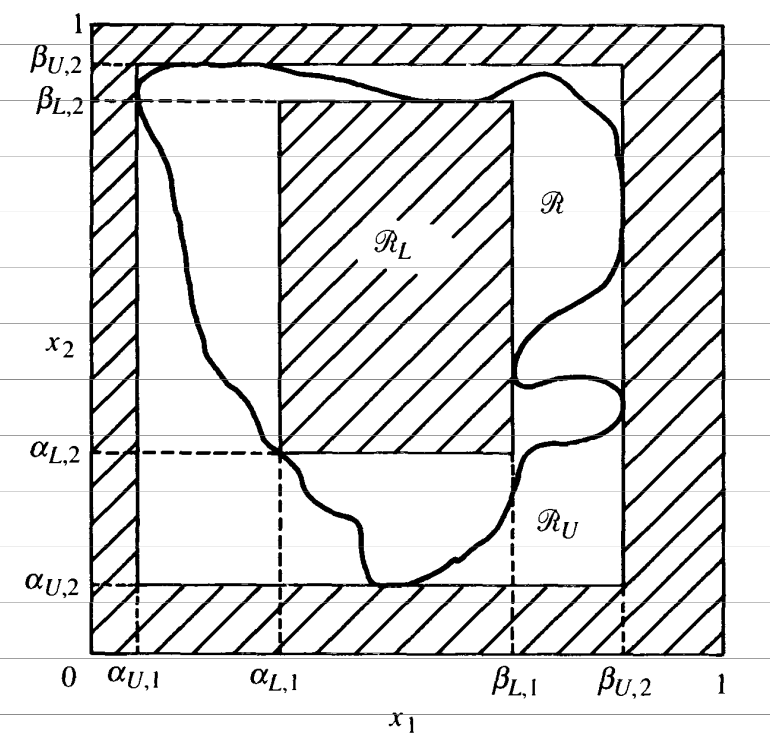
\includegraphics[width=0.7\textwidth]{images/hyperrectangle.png}
\caption{二维的矩形界:$\mathscr{R}_L \subseteq \mathscr{R} \subseteq
  \mathscr{R}_U \subseteq \mathscr{J}^2$。}
\label{fig::hyperrectangle2D}
\end{figure}

\begin{theorem}{}
  令
  \begin{equation}
    \phi_L(\vec{x}) = \left\{
    \begin{array}{ll}
      1,& \vec{x} \in \mathscr{R}_L\\
      0,& \mbox{其他}.
      \end{array}
      \right.
      \label{eq::sta_L}
  \end{equation}
  和
  \begin{equation}
  \phi_U(\vec{x}) = \left\{
  \begin{array}{ll}
    1,& \vec{x} \in \mathscr{R}_U\\
    0,& \mbox{其他}.
    \end{array}
    \right.
    \label{eq::sta_U}
  \end{equation}
  若$f(\vec{x})$表示在$\mathscr{J}^m$均匀分布的概率密度函数,令
  $\vec{X}$服从的概率密度函数为:
  \begin{equation}
    f(\vec{x}, \lambda_L, \lambda_U) = \frac{\phi_U(\vec{x}) -
      \phi_L(\vec{x})}{\lambda_U - \lambda_L}f(\vec{x}), \vec{x} \in
    \mathscr{J}^m.
    \label{eq::hyperrectangle_pdf}
  \end{equation}
  则
  \begin{equation}
    Z = \lambda_L + (\lambda_U - \lambda_L) \phi(\vec{X}),
    \label{eq::hyper_est}
  \end{equation}
  满足
  \begin{enumerate}
  \item
    \begin{equation}
      E[Z] = \lambda.
      \label{eq::hyper_exp}
    \end{equation}
  \item
    \begin{eqnarray}
      \mathrm{var} Z & = & (\lambda - \lambda_L)(\lambda_U - \lambda)
      \label{eq::hyper_var}
      \\
      & \leq & \frac{(\lambda_U - \lambda_L)^2}{4}. \notag
    \end{eqnarray}
  \end{enumerate}
    \label{thm::hyperrectangle}
\end{theorem}

这个定理的证明是简单的。定理中的$\phi(\vec{x})$的取值为
\begin{equation}
  \phi(\vec{x}) = \left\{
  \begin{array}{ll}
    1,& \vec{x} \in \mathscr{R}\\
    0,& \mbox{其他}.
  \end{array}
  \right.
  \label{eq::sta}
\end{equation}

接下去的问题如何产生服从$f(\vec{x}, \lambda_L,\lambda_U)$的随机数?办
法基本上有两种,一种是仍然产生在整个$\mathscr{J}^m$均匀分布的点,但是
用拒绝接受(AR)策略来过滤出落在$\mathscr{R}_L$和$\mathscr{R}_U$之间的
点。第二种是考虑整个$\mathscr{R}_U \backslash \mathscr{R}_L$区域被
$\alpha_{Li}$,$\alpha_{Ui}$,$\beta_{Li}$和$\beta_{Ui}$分成了$m$个区
域,每个区域由两个小超矩形块组成。我们可以先从这些块中,按体积为概率选
择一个,再在上面均匀投点,这样投点的计算量仍然是$\Theta(m)$的。这两种
策略的具体实现都参见参考书2.5节。其中第50页的Version C是上面的第二种思
路的$m$维一般化,见算法(\ref{alg::MC_bound_sample_directly})。

\begin{minipage}[!ht]{0.8\textwidth}
\vspace{3ex}
\refstepcounter{alg}
\label{alg::MC_bound_sample_directly}
\begin{center}
 算法 \arabic{chapter}.\arabic{alg} $m$维超矩形上下界约束下的直接抽取
\end{center}
\small
\begin{tabular}{ll}
  \hei 目标&对$\mathscr{R}_L \subseteq \mathscr{R}_U \subseteq \mathscr{J}^m$,
  直接抽取一个在$\mathscr{R}_U \backslash \mathscr{R}_L$中均匀分布的随机向量$\vec{X}$.\\
  \hei 输入&包含在
  $\mathscr{J}^m$中的超矩形区域$\mathscr{R}_L$和$\mathscr{R}_U$的顶点坐标数据
  $\alpha_{Lj}, \beta_{Lj}, \alpha_{Uj}, \beta_{Uj}$,\\
  &且$\mathscr{R}_L \subseteq \mathscr{R}_U$, $j = 1, 2, \cdots, m$.
\end{tabular}
\begin{enumerate}
\item 计算分块的体积(测度)$s_j$, $j = 1, 2, \cdots, m$, 并由此产生落入各分块的累计分布函数$t_j=\sum_{i=1}^j s_i$, $j = 1, 2, \cdots, m$. 
\item 产生一个服从$U(0, 1)$的随机数$Z$, 根据$Z$具体位置产生实际抽样分块
  $J \in \{1, 2, \cdots, m\}$, $t_{J-1} \leq Z < t_J$, $t_0 = 0$.
\item 计算$\Delta_1 = \beta_{UJ} - \beta_{LJ}$, $\Delta_2 = \alpha_{LJ} - \alpha_{UJ}$.
\item j = 1.
\item While $j < J$:
  \begin{enumerate}
    \item 产生服从$U(\alpha_{Lj}, \beta_{Lj})$的随机数$X_j$;
    \item j = j + 1.
  \end{enumerate}
\item 产生服从$U(0, 1)$的随机数$Y$,
  $$
  X_J = \beta_{LJ} + \left\lfloor(\Delta_1 + \Delta_2) Y / \Delta_1\right\rfloor
  (\alpha_{UJ} - \beta_{UJ}) + Y(\Delta_1 + \Delta_2).
  $$
\item j = j + 1.
\item While $j \leq m$:
  \begin{enumerate}
  \item 产生服从$U(\alpha_{Uj}, \beta_{Uj})$的随机数$X_j$.
  \item j = j + 1.
  \end{enumerate}
\end{enumerate}
\end{minipage}

在算法(\ref{alg::MC_bound_sample_directly})中,$s_j$的生成如下:令$a_i = \beta_{Li} - \alpha_{Li}$,$b_i = \beta_{Ui} - \alpha_{Ui}$,$1 \leq i \leq m$,
\begin{equation}
  s_j = \left\{
  \begin{array}{ll}
    \displaystyle (b_1 - a_1)\left(\prod_{i = 2}^m b_i\right) \cdot \frac{1}
    {\lambda_U - \lambda_L}, & j = 1\\\\
    \displaystyle \left(\prod_{i = 1}^{j - 1} a_i\right)(b_j - a_j)
    \left(\prod_{i = j + 1}^m b_i\right) \cdot \frac{1}{\lambda_U - \lambda_L}, &
    1 < j < m.\\\\
    \displaystyle (b_m - a_m)\left(\prod_{i = 1}^{m - 1}a_i\right) \cdot \frac{1}{\lambda_U - \lambda_L}, & j = m.
  \end{array}
  \right.
\end{equation}
其中
$$
\lambda_L = \prod_{i = 1}^m a_i, \lambda_U = \prod_{i = 1}^m b_i.
$$


而具体的MC算法相应修改为如下算法(\ref{alg::MC_S})。

\begin{minipage}[!ht]{0.8\textwidth}
\vspace{3ex}
\refstepcounter{alg}
\label{alg::MC_S}
\begin{center}
 算法 \arabic{chapter}.\arabic{alg} 在上下界估计下的MC方法
\end{center}
\small
\begin{tabular}{ll}
  \hei 目标&估算$\lambda(\mathscr{R})$.\\
  \hei 输入&包含在
  $\mathscr{J}^m$中的区域$\mathscr{R}$, $\lambda(\mathscr{R})$的下界估计$\lambda_L$
  和上界估计$\lambda_U$, 样本尺寸$n$, 置信水平$1 - \delta$. \\
  \hei 输出& 无偏点估计$\bar{\lambda}_n(\mathscr{R})$, 方差$\mathrm{var}
  \bar{\lambda}_n(\mathscr{R})$ 以及置信区间.
\end{tabular}
\begin{enumerate}
\item $j = 1$, $S = 0$.
\item While $j \leq n$:
  \begin{enumerate}
    \item 生成$\vec{X}^{(j)}$服从概率密度函数$f(\vec{x}, \lambda_L, \lambda_U)$.
    \item $\phi(\vec{X}^{(j)}) = 0$.
    \item If $\vec{X}^{(j)} \in \mathscr{R}, \phi(\vec{X}^{(j)}) = 1$.
    \item $S = S + \phi(\vec{X}^{(j)})$.
    \item j = j + 1.
  \end{enumerate}
\item 做统计分析:
  \begin{enumerate}
  \item 计算$\bar{\lambda}_n(\mathscr{R})
    = \lambda_L + (\lambda_U - \lambda_L)S/n$作为$\lambda(\mathscr{R})$的点估计.
  \item 计算$V[\bar{\lambda}_n(\mathscr{R})]
    = (\lambda_U - \lambda_L)^2(S / n)(1 - S / n) / (n - 1)$
    作为$\mathrm{var~} \bar{\lambda}_n(\mathscr{R})$的点估计.
  \item 根据置信水平计算百分之$100 \times (1 - \delta)$的置信区间:
    $$
    I_i(S, n, \delta) = \lambda_L + (\lambda_U - \lambda_L)\tilde{I_i},
    i = 1, 2.
    $$
    这里$\tilde{I_i}$是原MC中对应的置信区间界.
  \end{enumerate}
\end{enumerate}
\end{minipage}


\section{网络可靠性}

接下去我们讨论一个MC方法的应用例子。首先我们需要一点点图论的知识。令
$G$表示一个无向网络(undirected network),它的顶点(nodes)编号的集合是
$\mathscr{V}$,而全部边(edges)编号的集合是
$$
\mathscr{E} = \{1, 2, \cdots, m\}.
$$
我们现在考虑这个由顶点和边组成的网络,假设全部的顶点都是可靠的,但边
的可靠性却是一个独立的随机事件。也即$\forall i \in \mathscr{E}$,这条
边连通的概率是$q_i$,而有$1 - q_i$的概率是不连通的。现在用随机变量$y_i$
表示一条边是否连通的状态,也即
$$
y_i = \left\{
\begin{array}{ll}
  1, & \mbox{边$i$是连通的};\\
  0, & \mbox{其它}.
\end{array}
\right.
$$
则$\vec{y} = (y_1, y_2, \cdots, y_m)$表示整个网络$m$条边的状态。用
$\mathscr{Y}$表示全部$\vec{y}$可能状态的集合。

$\forall s, t \in \mathscr{V}$,令
$$
\phi(\vec{y}) = \left\{
\begin{array}{ll}
  1, & \mbox{若$s$和$t$在$\vec{y}$状态下是连通的}.\\
  0, & \mbox{其它}.
\end{array}
\right.
$$

\begin{figure}[!ht]
  \centering
    \begin{tikzpicture}
	\path [use as bounding box] (-4,-2.25) rectangle (4,5.5);
	\begin{pgfonlayer}{nodelayer}
		\node [style=wn] (0) at (-1, 3) {1};
		\node [style=wn] (1) at (1, 3) {2};
		\node [style=wn] (2) at (-1.5, 1.5) {5};
		\node [style=wn] (3) at (1.5, 1.5) {3};
		\node [style=wn] (4) at (3, 1.25) {9};
		\node [style=wn] (5) at (0, 1.75) {6};
		\node [style=wn] (6) at (-2, 4.25) {7};
		\node [style=wn] (7) at (2, 4.25) {8};
		\node [style=wn] (8) at (0, 0.25) {4};
		\node [style=wn] (9) at (0, -1.25) {10};
		\node [style=wn] (10) at (-3, 1.25) {11};
		\node [style=none] (11) at (-0.25, 2.5) {1};
		\node [style=none] (12) at (0.25, 2.5) {2};
		\node [style=none] (13) at (0.75, 2) {3};
		\node [style=none] (14) at (0.25, 1) {4};
		\node [style=none] (15) at (-0.75, 2) {5};
		\node [style=none] (16) at (0, 3.25) {6};
		\node [style=none] (17) at (1.5, 2.25) {7};
		\node [style=none] (18) at (1, 0.75) {8};
		\node [style=none] (19) at (-1, 0.75) {9};
		\node [style=none] (20) at (-1.5, 2.25) {10};
		\node [style=none] (21) at (1.5, 3.25) {11};
		\node [style=none] (22) at (2.25, 1.75) {12};
		\node [style=none] (23) at (0.25, -0.5) {13};
		\node [style=none] (24) at (-2.25, 1.75) {14};
		\node [style=none] (25) at (-1.5, 3.25) {15};
		\node [style=none] (26) at (0, 4.5) {16};
		\node [style=none] (27) at (2.75, 2.75) {17};
		\node [style=none] (28) at (2, -0) {18};
		\node [style=none] (29) at (-1.75, -0.25) {19};
		\node [style=none] (30) at (-2.75, 3) {20};
	\end{pgfonlayer}
	\begin{pgfonlayer}{edgelayer}
		\draw (0) to (1);
		\draw (6) to (0);
		\draw (7) to (1);
		\draw (0) to (5);
		\draw (5) to (1);
		\draw (2) to (5);
		\draw (5) to (3);
		\draw (5) to (8);
		\draw (2) to (8);
		\draw (8) to (3);
		\draw (3) to (1);
		\draw (0) to (2);
		\draw (10) to (2);
		\draw (9) to (8);
		\draw (3) to (4);
		\draw (4) to (7);
		\draw (7) to (6);
		\draw (6) to (10);
		\draw (10) to (9);
		\draw (9) to (4);
	\end{pgfonlayer}
    \end{tikzpicture}
\caption{一个网络的示意图}
\end{figure}

再令
$$
P(\vec{y}, \vec{q}) = \prod_{i \in \mathscr{E}} q_i^{y_i}(1 - q_i)^{1 - y_i},
$$
其中
$$
\vec{q} = (q_1, \cdots, q_m),
$$
则我们关心的是$s$和$t$之间连通的概率,也即
\begin{equation}
  g(\vec{q}) = \sum_{\vec{y} \in \mathscr{Y}} \phi(\vec{y}) P(\vec{y}, \vec{q}).
\end{equation}
如果$\vec{q}$是已知的,那么$g(\vec{q})$是可计算的(computable)。它应该就严格等于
\begin{equation}
  g(\vec{q}) = \sum_{\vec{y} \in \mathscr{Y}_1} P(\vec{y}, \vec{q}),
  \label{eq::network_relia}
\end{equation}
其中
$$
\mathscr{Y}_1 = \{\vec{y} \in \mathscr{Y} \left| \phi(\vec{y}) = 1\right.\}.
$$


然而,如何确定$\mathscr{Y}_1$是一个NP-Hard的问题
\cite{Provan1984Computing}。在这种情况下,MC方法也成为一个进行计算模拟
的有效手段。

用$\Gamma$表示网络$G$中点$s-t$的最小切割集(minimal $s-t$ cutsets)全体。
一个$s-t$的切割集是一些边的集合,在$G$中去除这些边,就会使$s-t$不再连
通。而最小切割集则表示该集合的任何子集都不会切割$s-t$。于是
$$
\begin{array}{rcl}
\displaystyle \phi(\vec{y}) &=& \displaystyle \prod_{\mathscr{C} \in
  \Gamma} \left[1 - \prod_{i \in \mathscr{C}}(1 - y_i)\right] \\\\ & =
& \displaystyle \prod_{\mathscr{C} \in \Gamma}\left[1 - \min_{i \in
    \mathscr{C}}(1 - y_i)\right].
\end{array}
$$
令$x_i \in [0, 1]$,$i \in \mathscr{E}$,则可取
$$
y_i = 1 - \lfloor 1 - q_i + x_i \rfloor.
$$
于是$s-t$网络可靠性(\ref{eq::network_relia})等价于计算区域
$$
\mathscr{R} = \left\{(x_1, \cdots, x_m) \in \mathscr{J}^m
\left| \min_{\mathscr{C} \in \Gamma} \left[1
  - \min_{i \in \mathscr{C}}(\lfloor1 - q_i + x_i\rfloor)\right] = 1\right.\right\}.
$$

我们可以用MC方法求解这个面积。同样地,为了提高采样精度,我们可以来考虑
$\lambda_L$和$\lambda_U$。也就是$\mathscr{R}$的上下界估计,同时这种估
计还要能够满足简单采样的要求。

我们用$\mathscr{P}_1, \mathscr{P}_2, \cdots, \mathscr{P}_I$表示网络$G$
的全部$I$个$s-t$不相交最短路径集(edge-disjoint paths),即
$\forall i \in \{1, 2, \cdots, I\}$,$\mathscr{P}_i$中的边构成$s$到$t$
在$G$中的最短路径,且$\mathscr{P}_i \cap \mathscr{P}_j = \emptyset$,
$\forall i \neq j$。类似地,记$\mathscr{C}_1, \mathscr{C}_2, \cdots,
\mathscr{C}_J$为$J$个$G$中的$s-t$不相交最小切割集(edge-disjoint
  minimal $s-t$ cutsets)。令
$$
\phi_L(\vec{y}) = \left\{
\begin{array}{ll}
  1, & \mbox{若$\vec{y}$在至少在一个不相交最短路径集上全部连通},\\
  0, & \mbox{其他}.
\end{array}
\right.
$$
(若$\phi_L(\vec{y}) = 1$则$s-t$必然连通。)类似地,令
$$
\phi_U(\vec{y}) = \left\{
\begin{array}{ll}
  1, & \mbox{若$\vec{y}$在每个不相交最小切割集中都至少有一条边连通},\\
  0, & \mbox{其他}.
\end{array}
\right.
$$
(若$\phi_U(\vec{y}) = 0$则说明至少有一个不相交最小切割集完成了切割,
  因此$s-t$必然分离。)等价地,
\begin{equation}
  \begin{array}{rcl}
\phi_L(\vec{y}) &=& \displaystyle 1 - \prod_{j = 1}^I\left(1 - \prod_{i \in
  \mathscr{P}_j} y_i\right), \\
\phi_U(\vec{y}) &=& \displaystyle \prod_{j = 1}^J\left(1 - \prod_{i \in
  \mathscr{C}_j} (1 - y_i)\right).
  \end{array}
  \label{eq::network_phi_lu}
\end{equation}

注意到必然有$\phi_L(\vec{y}) \leq \phi(\vec{y}) \leq \phi_U(\vec{y})$,于是可构建
\begin{equation}
  \begin{array}{rcl}
  g_L(\vec{q}) &=&\displaystyle \sum_{\vec{y} \in \mathscr{Y}}
  \phi_L(\vec{y}) P(\vec{y}, \vec{q}),\\ &=&\displaystyle 1 - \prod_{j
    = 1}^I\left(1 - \prod_{i \in \mathscr{P}_j}q_i\right)
  \end{array}
  \label{eq::network_gl}
\end{equation}
和
\begin{equation}
  \begin{array}{rcl}
  g_U(\vec{q}) &=&\displaystyle \sum_{\vec{y} \in \mathscr{Y}}
  \phi_U(\vec{y}) P(\vec{y}, \vec{q}),\\ &=&\displaystyle
  \prod_{j = 1}^J\left(1 - \prod_{i \in \mathscr{C}_j}(1 - q_i)\right)
  \end{array}
  \label{eq::network_gu}
\end{equation}
作为MC方法估算$g(\vec{q})$的上下界。这个估算是重要的,因为显然,满足
$\phi_U(\vec{y}) = 1$的$\vec{y}$要比$\vec{y}$的全部$2^m$种组合少得多。
因此这种界的约束可以极大地降低模拟结果的方差。类似(\ref{eq::hyperrectangle_pdf}),
我们可以构建概率密度函数
\begin{equation}
  P(\vec{y}, \vec{q}, \lambda_L, \lambda_U) = \frac{\phi_U(\vec{y}) -
    \phi_L(\vec{y})}{g_U(\vec{q}) - g_L(\vec{q})}P(\vec{y}, \vec{q}), \vec{y}
  \in \mathscr{Y}.
  \label{eq::network_bound_pdf}
\end{equation}
若随机向量$\vec{Y}$服从$P(\vec{y}, \vec{q}, \lambda_L, \lambda_U)$,则
\begin{equation}
  \psi(\vec{Y}) = g_L(\vec{q}) + (g_U(\vec{q}) - g_L(\vec{q})) \phi(\vec{Y})
  \label{eq::network_bound_estimate_g}
\end{equation}
的期望是$g(\vec{q})$且
\begin{equation}
  \begin{array}{rcl}
  \mathrm{var} \phi(\vec{Y}) &=& (g_U(\vec{q}) - g(\vec{q}))
  (g(\vec{q}) - g_L(\vec{q}))\\
  & \leq& \displaystyle \frac{(g_U(\vec{q}) - g_L(\vec{q}))^2}{4}.
  \end{array}
  \label{eq::network_bound_estimate_var}
\end{equation}

现在总结一下MC模拟网络可靠性的算法,即算法\ref{alg::MC_Network}。

\begin{minipage}[!ht]{0.8\textwidth}
\vspace{3ex}
\refstepcounter{alg}
\label{alg::MC_Network}
\begin{center}
 算法 \arabic{chapter}.\arabic{alg} 估算$s-t$网络可靠性$g(\vec{q})$
\end{center}
\small
\begin{tabular}{ll}
  \hei 目标&估算$g(\vec{q})$.\\
  \hei 输入& 网络$G = (\mathscr{V}, \mathscr{E})$, 起点$s$, 终点$t$,
  网络可靠性向量$\vec{q}$, 置信水平$1-\delta$. \\
  \hei 输出& $g(\vec{q})$的无偏点估计$\hat{g}_n(\vec{q})$,
  $\mathrm{var} \hat{g}_n(\vec{q})$,  以及关于$\delta$的置信区间.
\end{tabular}
\begin{enumerate}
\item 计算$g_L(\vec{q})$和$g_U(\vec{q})$.
\item $j = 1$, $S = 0$.
\item While $j \leq n$:
  \begin{enumerate}
  \item 生成$\vec{Y} = (Y_1, \cdots, Y_m)$服从概率密度函数
    $P(\vec{y}, \vec{q}, \lambda_L, \lambda_U)$.
    \item $\phi(\vec{Y}) = 0$.
    \item If $s$ 和 $t$ 连通,$\phi(\vec{Y}) = 1$.
    \item $S = S + \phi(\vec{Y})$.
    \item j = j + 1.
  \end{enumerate}
\item 做统计分析:
  \begin{enumerate}
  \item 计算$\hat{g}_n(\vec{q}) = g_L(\vec{q}) + [g_U(\vec{q}) -
    g_L(\vec{q})] S/n$作为$g(\vec{q})$的点估计.
  \item 计算$V[\hat{g}_n(\vec{q})] = (g_U(\vec{q}) -
    \hat{g}_n(\vec{q}))(\hat{g}_n(\vec{q}) - g_L(\vec{q})) / (n -1)$作
    为$\mathrm{var} \hat{g}_n(\vec{q})$的点估计.
  \item 根据置信水平计算百分之$100 \times (1 - \delta)$的置信区间:
    $$
    I_i(S, n, \delta) = g_L(\vec{q}) + (g_U(\vec{q}) - g_L(\vec{q}))\tilde{I_i},
    i = 1, 2.
    $$
    这里$\tilde{I_i}$是原MC中对应的置信区间界.
  \end{enumerate}
\end{enumerate}
\end{minipage}

算法\ref{alg::MC_Network}还有几个细节没有说明,首先是如何产生
$\mathscr{P}_i$和$\mathscr{C}_i$集合,以及如何判定在$G$中的两点$s$和$t$
是否连通。这些是涉及图论的算法,资料很多,大家自己查阅。其次是如何产生
分布$P(\vec{y}, \vec{q}, \lambda_L, \lambda_U)$,由于问题复杂,参考书
建议直接采用AR方法,也即先根据$\vec{q}$随机产生$\vec{y}$,然后拒绝
$\phi_U(\vec{y}) = 0$和$\phi_L(\vec{y}) = 1$的样本。如何直接产生满足要
求的样本是一个可以考虑的问题。但这个问题有一定的深度和难度。

\section{Monte Carlo积分}

积分问题可以看成是求面积问题的一般化。但其重要性使得我们需要单独讨论这个问
题。考虑多元积分问题:
\begin{equation}
  \zeta(\mathscr{R}) = \int_{\mathscr{R}}\varphi(\vec{x}) d\vec{x},
  \label{eq::mc_integeration}
\end{equation}
其中$\varphi(\vec{x})$是定义在$m$维区域$\mathscr{R} \subseteq \mathscr{J}^m$
上的可求值的Lebesgue可积函数。为方便讨论,我们令$\varphi(\vec{x}) = 0$,
对$\vec{x} \in \mathscr{J}^m \backslash \mathscr{R}$。

先考虑一维积分问题
$$
I = \int_a^b f(x) dx,
$$
我们的经典数值积分方法是通过数值积分公式:
$$
I_n = \sum_{i = 0}^n w_if(x_i),
$$
其中$w_i$称为积分权重,而$a \leq x_0 \leq x_1 \leq \cdots \leq x_n
\leq b$被称为积分点。现在让我们类似地考虑,将$[a, b]$分割成$n$个等长的小区间,
记为$\Delta_1, \Delta_2, \cdots, \Delta_n$,每一个小区间的长度都是$(b - a) / n$。
记$\Delta_i$的中点为$x_{i + \frac{1}{2}}$,令$f_{i + \frac{1}{2}} := f(x_{i + \frac{1}{2}})$,$i = 1, 2, \cdots, n$。
则一方面由可积性定义,我们有
\begin{equation}
  \tilde{I}_n := \sum_{i = 1}^n \frac{b - a}{n}f_{i + \frac{1}{2}} \to I, n \to \infty.
  \label{eq::MC_integeration_eI}
\end{equation}
另一方面,构造$f(x)$的分段常数逼近:
\begin{equation}
  \tilde{f}_n(x) = f_{i + \frac{1}{2}}, x \in \Delta_i, i = 1, 2, \cdots, n.
  \label{eq::MC_approximation_kernel}
\end{equation}
则显然$\tilde{f}_n(x) \stackrel{\mathrm{\tiny a. e.}}\longrightarrow  f(x)$, $n \to \infty$。
现在对于随机变量$X \sim U(a, b)$,我们定义指示随机变量
$$
 \phi_i(X) = \left\{
 \begin{array}{ll}
   1, & \mbox{如果$X$落在区间$\Delta_i$上};\\
   0, & \mbox{其他}.
 \end{array}
 \right.
 $$
这里$i = 1, 2, \cdots, n$,则有
$$
\tilde{f}_n(X) = \sum_{i = 1}^n \phi_i(X) f_{i + \frac{1}{2}}.
$$
于是
$$
\begin{array}{rcl}
  E[\tilde{f}_n(X)] &=& \displaystyle E\left[\sum_{i = 1}^n \phi_i(X) f_{i + \frac{1}{2}}\right]\\\\
  &=& \displaystyle \sum_{i = 1}^n \frac{1}{n} f_{i + \frac{1}{2}} \\\\
  &=& \displaystyle \frac{1}{n}\sum_{i = 1}^nf_{i + \frac{1}{2}}
\end{array}
$$
结合(\ref{eq::MC_integeration_eI})有
$$
\tilde{I}_n = (b - a) E[\tilde{f}_n(X)].
$$
两边同取$n \to \infty$,则有
\begin{equation}
  I = (b - a) E[f(X)].
  \label{eq::MC_integeration_source}
\end{equation}
因此,对$X_1, X_2, \cdots, X_n \sim U(a, b)$,
\begin{equation}
  I_n := \frac{b - a}{n} \sum_{i = 1}^n f(X_i).
  \label{eq::MC_integeration_estimation}
\end{equation}
可以看做是$I$的一个无偏估计。

该结论可以推广到$m$维。令$\vec{X}^{(1)}, \cdots, \vec{X}^{(n)}$是$m$维
独立随机向量,且在$\mathscr{J}^m$上均匀分布。则
\begin{equation}
  \bar{\zeta}_n(\mathscr{R}) = \frac{1}{n} \sum_{i = 1}^n \varphi(\vec{X}^{(i)})
  \label{eq::bar_zeta_n}
\end{equation}
是(\ref{eq::mc_integeration})中$\zeta(\mathscr{R})$的一个无偏估计,且
\begin{equation}
  \mathrm{var} \bar{\zeta}_n = \frac{\sigma^2}{n},
  \label{eq::var_zeta_n}
\end{equation}
这里
\begin{equation}
  \sigma^2 = \mathrm{var} \varphi(\vec{X}) = \int_{\mathscr{R}} \varphi^2(\vec{x})dx - \zeta^2.
  \label{eq::zeta_sigma_2}
\end{equation}
注意$\sigma^2$计算困难,所以可以用
\begin{equation}
  \hat{\sigma}^2_n = \frac{1}{n - 1}\sum_{j = 1}^n\left[\varphi(\vec{X}^{(j)}) - \bar{\zeta}_n\right]^2
  \label{eq::zeta_hat_sigma_2_store}
\end{equation}
来近似。然而,此公式要求存下所有的$\varphi(\vec{X})$,才能最终和
$\bar{\zeta}_n$进行计算,当$n$大时,对存储量要求高。常用的替代方案是利用其代数等价表达式
\begin{equation}
  \hat{\sigma}^2_n = \frac{1}{n - 1}\left[\sum_{j = 1}^n \varphi^2(\vec{X}^{(j)}) - n \bar{\zeta}^2_n\right].
  \label{eq::zeta_hat_sigma_2_encount}
\end{equation}

而对于区间估计,我们直接给出以下结果:当
\begin{equation}
  \int_{\mathscr{R}} \varphi^4(\vec{x}) d\vec{x} < \infty
\end{equation}
时,有
$$
\frac{\bar{\zeta}_n - \zeta}{\sqrt{\frac{\hat{\sigma}^2_n}{n}}}
$$
当$n \to \infty$时趋于服从$N(0, 1)$分布, 也即
\begin{equation}
  \lim_{n \to \infty} P\left\{\frac{\bar{\zeta}_n - \zeta}{\sqrt{\frac{\hat{\sigma}^2_n}{n}}} \leq \beta\right\} = \Phi(\beta).
\end{equation}
其中$\Phi$表示标准正态分布。故可以认为对充分大的$n$,区间
\begin{equation}
  \left[\bar{\zeta}_n - \Phi^{-1}\left(1 - \frac{\delta}{2}\right)\sqrt{\frac{\hat{\sigma}^2_n}{n}},
    \bar{\zeta}_n + \Phi^{-1}\left(1 - \frac{\delta}{2}\right)\sqrt{\frac{\hat{\sigma}^2_n}{n}}\right]
\end{equation}
以概率$1 - \delta$覆盖了$\zeta$。

类似面积计算,在积分计算时,我们同样应该考虑最低样本数、上下界、各种有
效抽样以及和网络等应用问题的关系这些基本问题。限于时间我们不再课堂展开
讨论,请大家自行参考书本的第二章的剩余部分和习题。


\bibliographystyle{plain}
\bibliography{crazyfish}
\end{document}
